\documentclass[
  % -- opções da classe memoir --
  12pt,     % tamaho da fonte
  openright,      % capítulos começam em págína ímpar
  oneside,      % para impressão em recto e verso. Oposto a oneside
  a4paper     % tamanho do papel        % o último idioma é o principal do documento
  ]{abntex2}

% ---
% Pacotes básicos
% ---
\usepackage{lmodern}      % Usa a latin modern
\usepackage[T1]{fontenc}		% Selecao de codigos de fonte.
\usepackage[utf8]{inputenc}		% Codificacao do documento (conversão automática dos acentos)
\usepackage{color}				% Controle das cores
\usepackage{microtype} 			% para melhorias de justificação
\usepackage{graphicx}
\usepackage{float}
% ---

% ---
% Pacotes de citações
% ---
\usepackage[brazilian,hyperpageref]{backref}	 % Paginas com as citações na bibliografia
\usepackage[alf]{abntex2cite}	% Citações padrão ABNT
% ---

% ---
% Configurações do pacote backref
% Usado sem a opção hyperpageref de backref
\renewcommand{\backrefpagesname}{Citado na(s) página(s):~}
% Texto padrão antes do número das páginas
\renewcommand{\backref}{}
% Define os textos da citação
\renewcommand*{\backrefalt}[4]{
	\ifcase #1 %
		Nenhuma citação no texto.%
	\or
		Citado na página #2.%
	\else
		Citado #1 vezes nas páginas #2.%
	\fi}%
% ---

% ---------------------------------------------
% Ajusta título das referências bibliográficas
% ---------------------------------------------
\renewcommand\bibsection{\chapter{\bibname}}

% ---
% Informações de dados para CAPA e FOLHA DE ROSTO
% ---
\titulo{Primeira lista de exercícios}
\autor{Ronaldo Costa de Freitas}
\local{Manaus, Amazonas}
\data{2021}
\orientador{prof. Hiram Carlos Costa Amaral}
\instituicao{
  Universidade do Estado do Amazonas -- UEA
  \par
  Faculdade de Sistemas de Informação}
% O preambulo deve conter o tipo do trabalho, o objetivo,
% o nome da instituição e a área de concentração
\preambulo{Trabalho acadêmico apresentado à Faculdade de Sistemas de Informação da Universidade do Estado do Amazonas como requisito para obtenção de nota parcial à matéria de Matemática Básica ministrada pelo prof. Hiram Carlos Costa Amaral.}
% ---

% ---
% Configurações de aparência do PDF final

% alterando o aspecto da cor azul
\definecolor{blue}{RGB}{41,5,195}

% informações do PDF
\makeatletter
\hypersetup{
     	%pagebackref=true,
		pdftitle={\@title},
		pdfauthor={\@author},
    	pdfsubject={\imprimirpreambulo},
	    pdfcreator={LaTeX with abnTeX2},
		pdfkeywords={abnt}{latex}{abntex}{abntex2}{trabalho acadêmico},
		colorlinks=true,       		% false: boxed links; true: colored links
    	linkcolor=blue,          	% color of internal links
    	citecolor=blue,        		% color of links to bibliography
    	filecolor=magenta,      		% color of file links
		urlcolor=blue,
		bookmarksdepth=4
}
\makeatother
% ---

% ---
% Espaçamentos entre linhas e parágrafos
% ---

% O tamanho do parágrafo é dado por:
\setlength{\parindent}{1.3cm}

% Controle do espaçamento entre um parágrafo e outro:
\setlength{\parskip}{0.2cm}  % tente também \onelineskip

% ---
% compila o indice
% ---
\makeindex
% ---

% ----
% Início do documento
% ----
\begin{document}

% Seleciona o idioma do documento (conforme pacotes do babel)
%\selectlanguage{english}
\selectlanguage{brazil}

% Retira espaço extra obsoleto entre as frases.
\frenchspacing

% ----------------------------------------------------------
% ELEMENTOS PRÉ-TEXTUAIS
% ----------------------------------------------------------
%\pretextual

% ---
% Capa
% ---
\imprimircapa
% ---

% ---
% Folha de rosto
% ---
\imprimirfolhaderosto
% ---

% ---
% inserir o sumario
% ---
\pdfbookmark[0]{\contentsname}{toc}
\tableofcontents*
\cleardoublepage
% ---

% ----------------------------------------------------------
% ELEMENTOS TEXTUAIS
% ----------------------------------------------------------
\textual

% ------------------------------------------------------------
% Capítulo da Introdução
% ------------------------------------------------------------
% ------------------------------------------------------------
% Capítulo da lista de exercícios
% ------------------------------------------------------------
\chapter{Resolução da lista de exercícios}

% ------------------------------------------------------------
% Exercícios da Série A
% ------------------------------------------------------------
\section{Série A}
%\addcontentsline{toc}{section}{Contribuições de Alan Turing à Ciência da Computação}
% ------------------------------------------------------------
\begin{figure}[H]
  \centering
  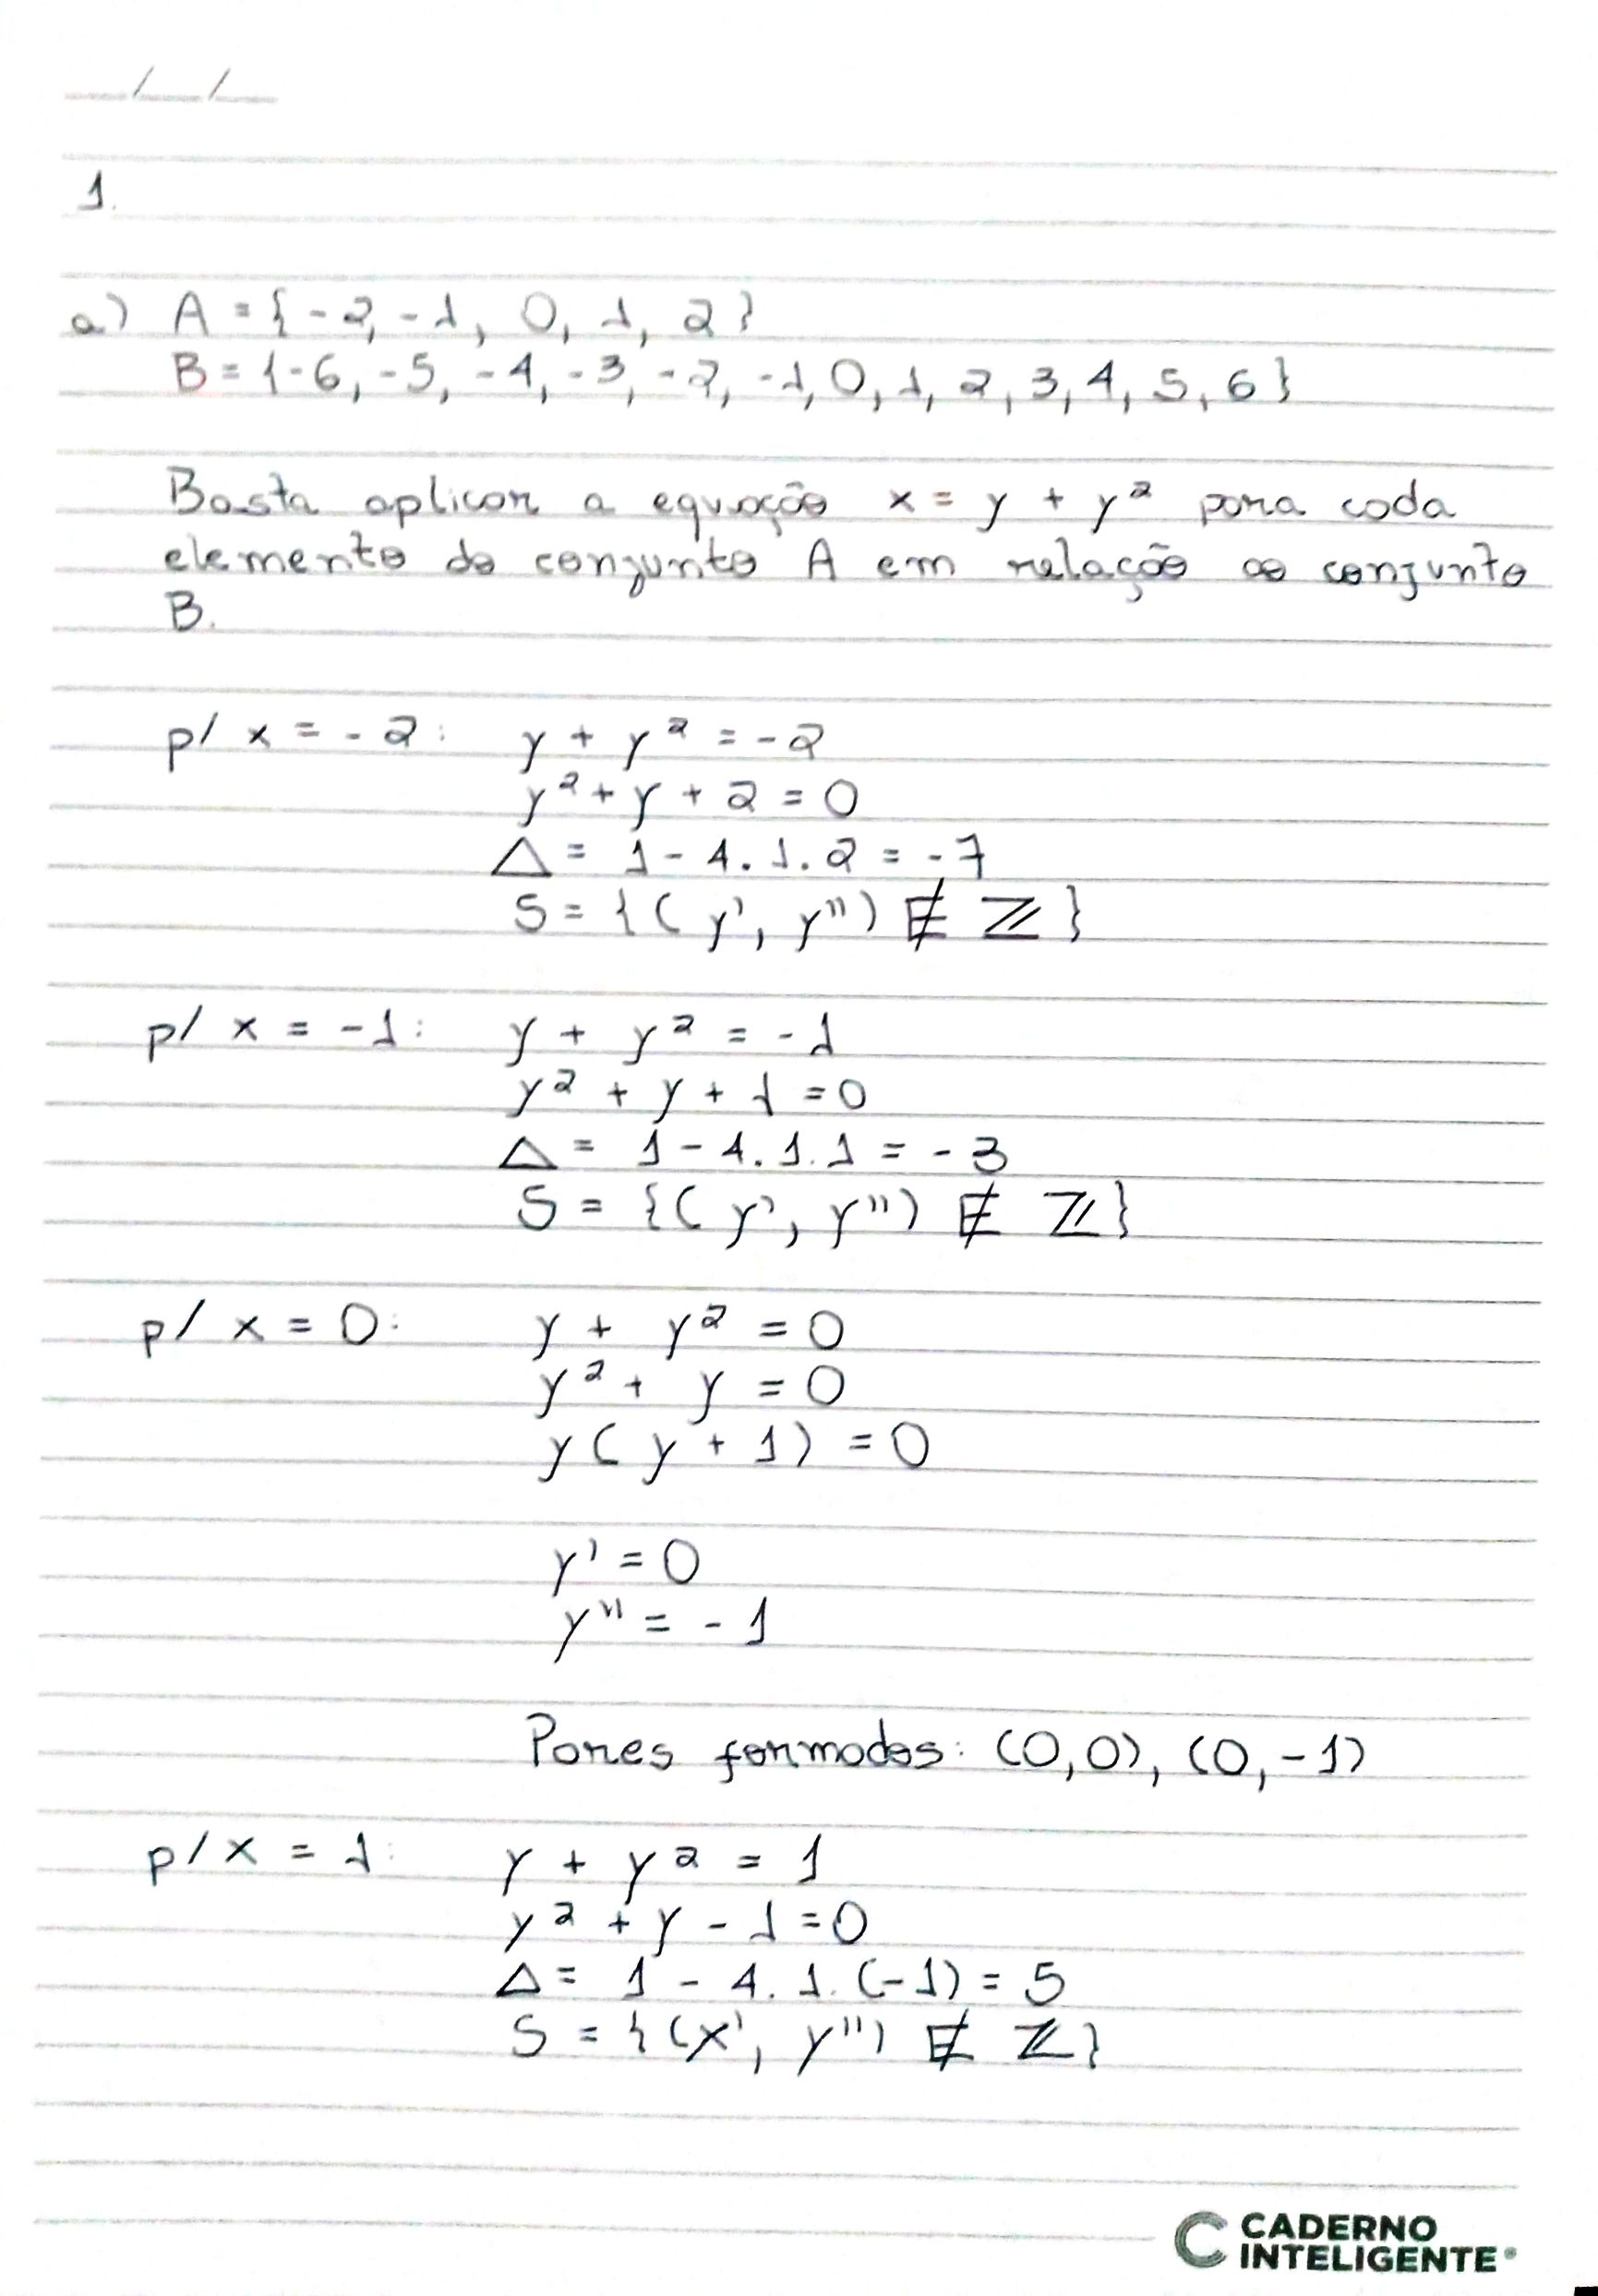
\includegraphics[scale=0.23]{pagina1.jpg}
\end{figure}

\begin{figure}[H]
  \centering
  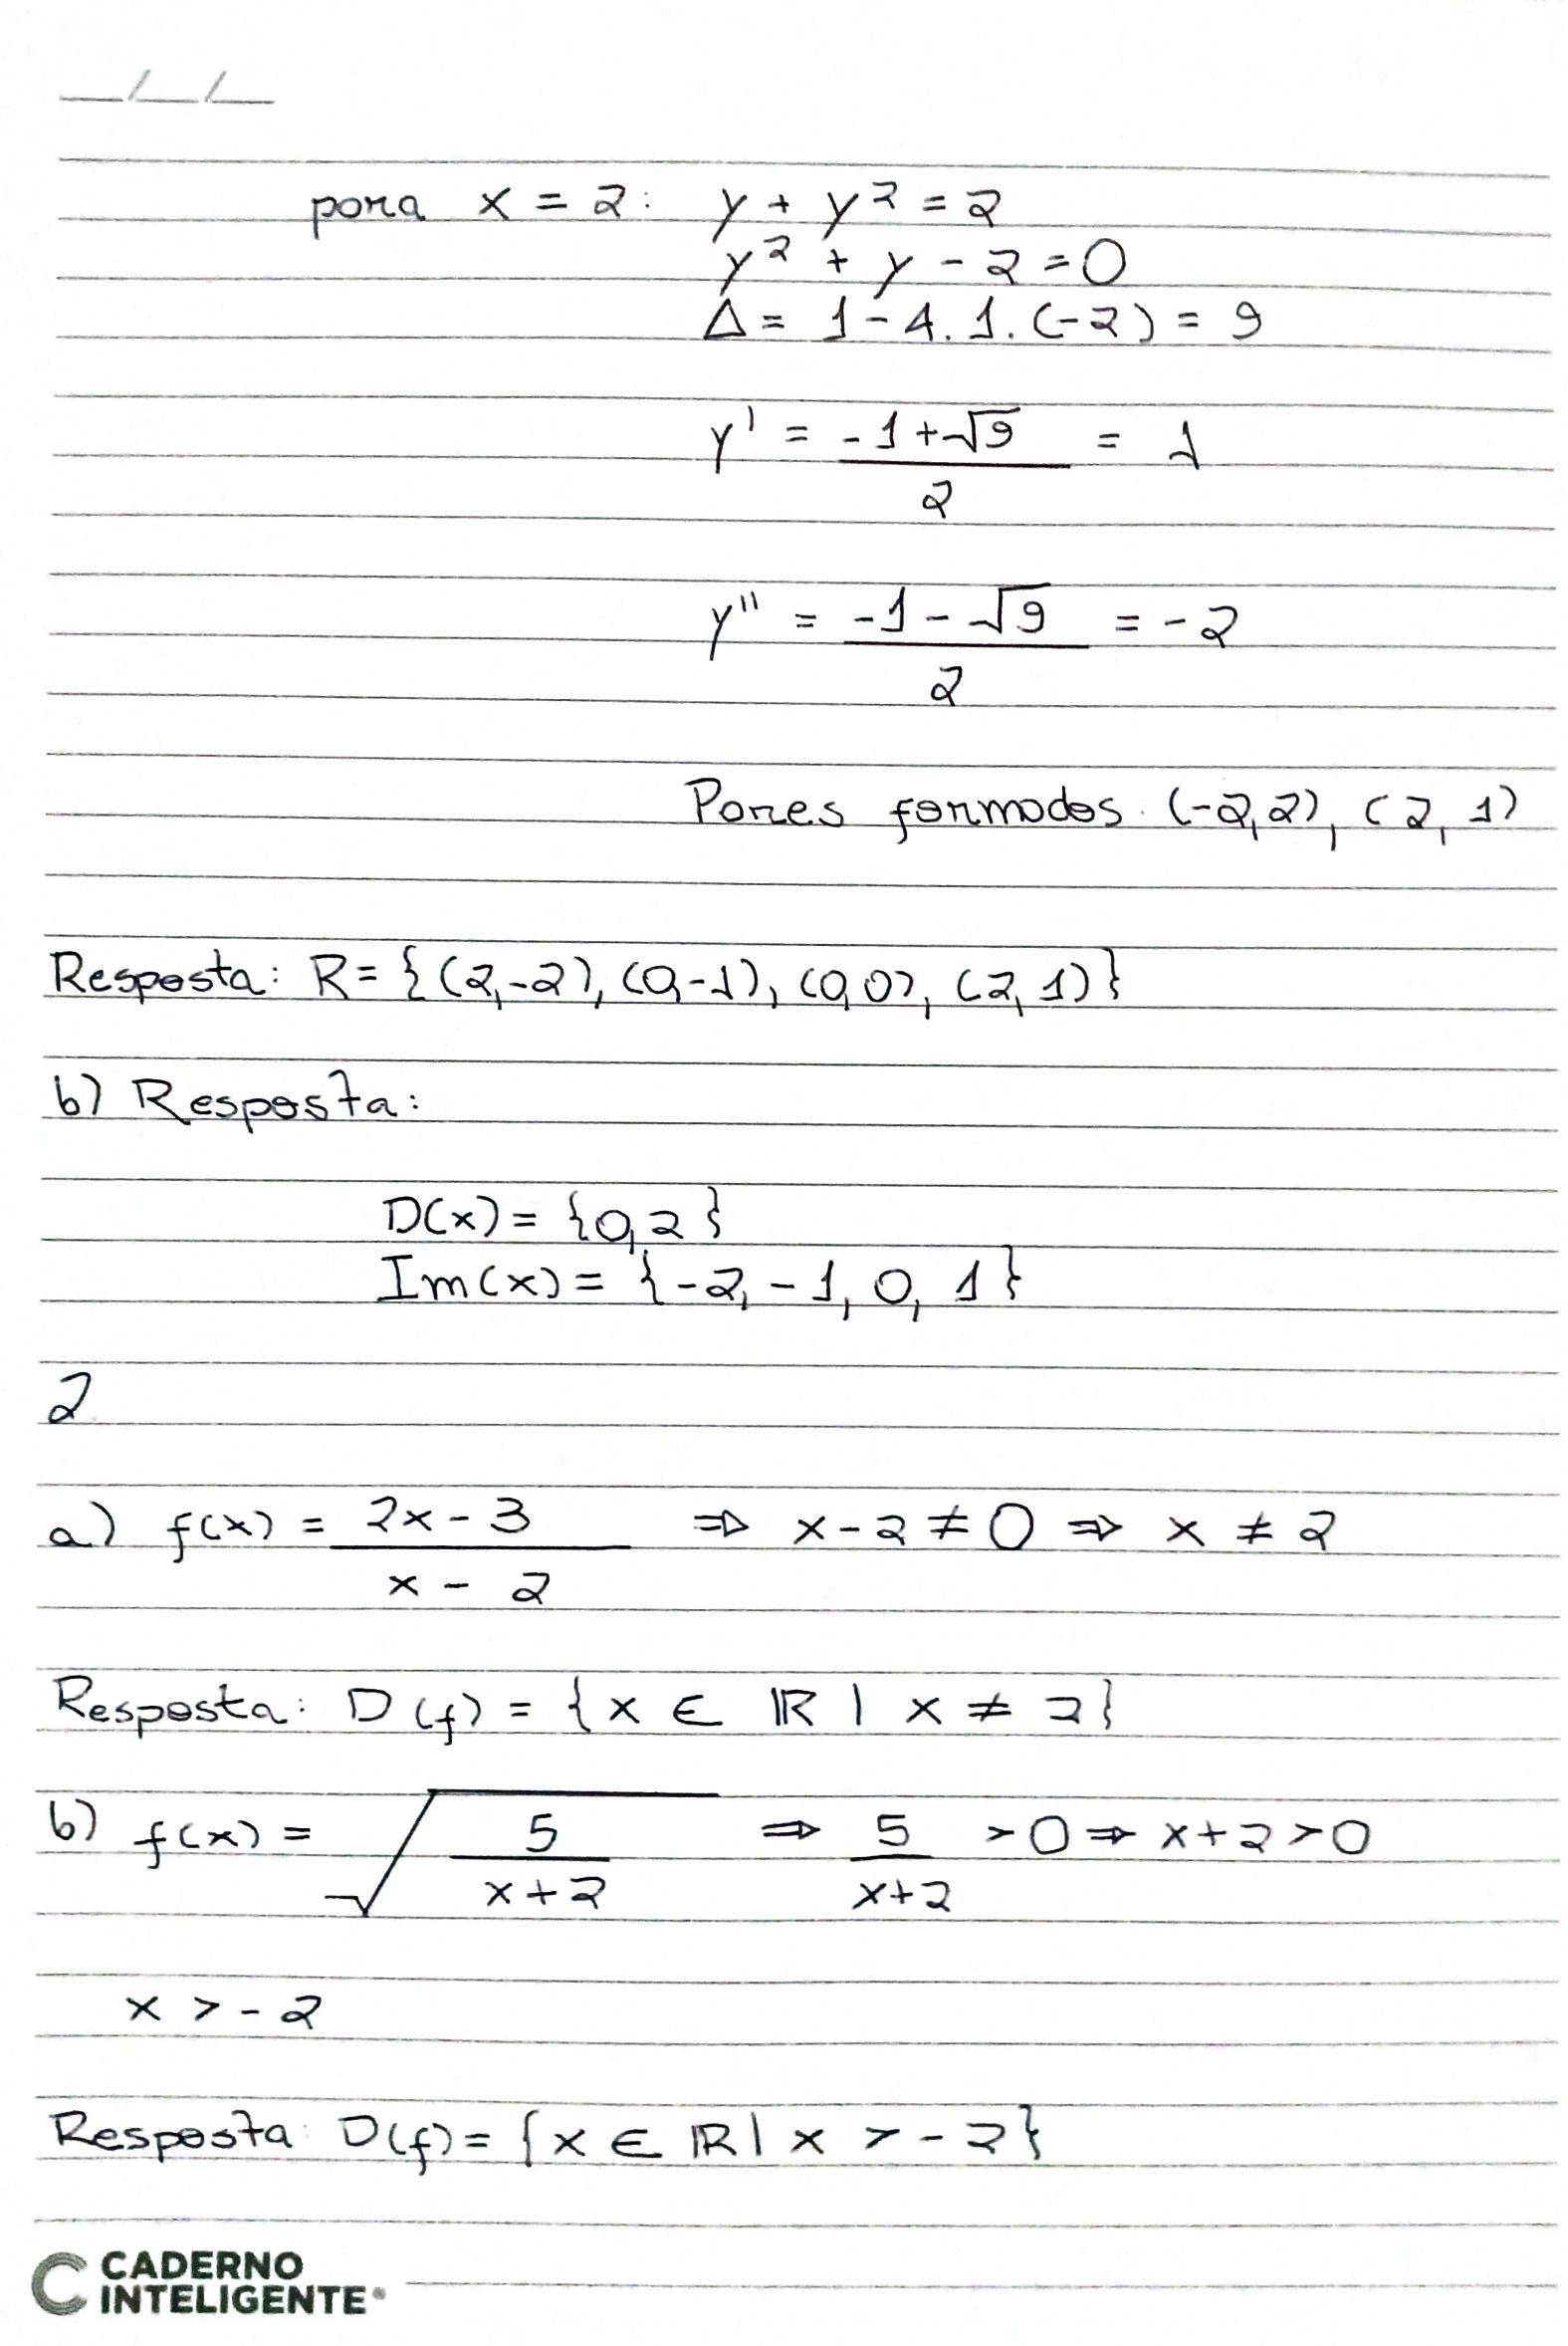
\includegraphics[scale=0.23]{pagina2.jpg}
\end{figure}

\begin{figure}[H]
  \centering
  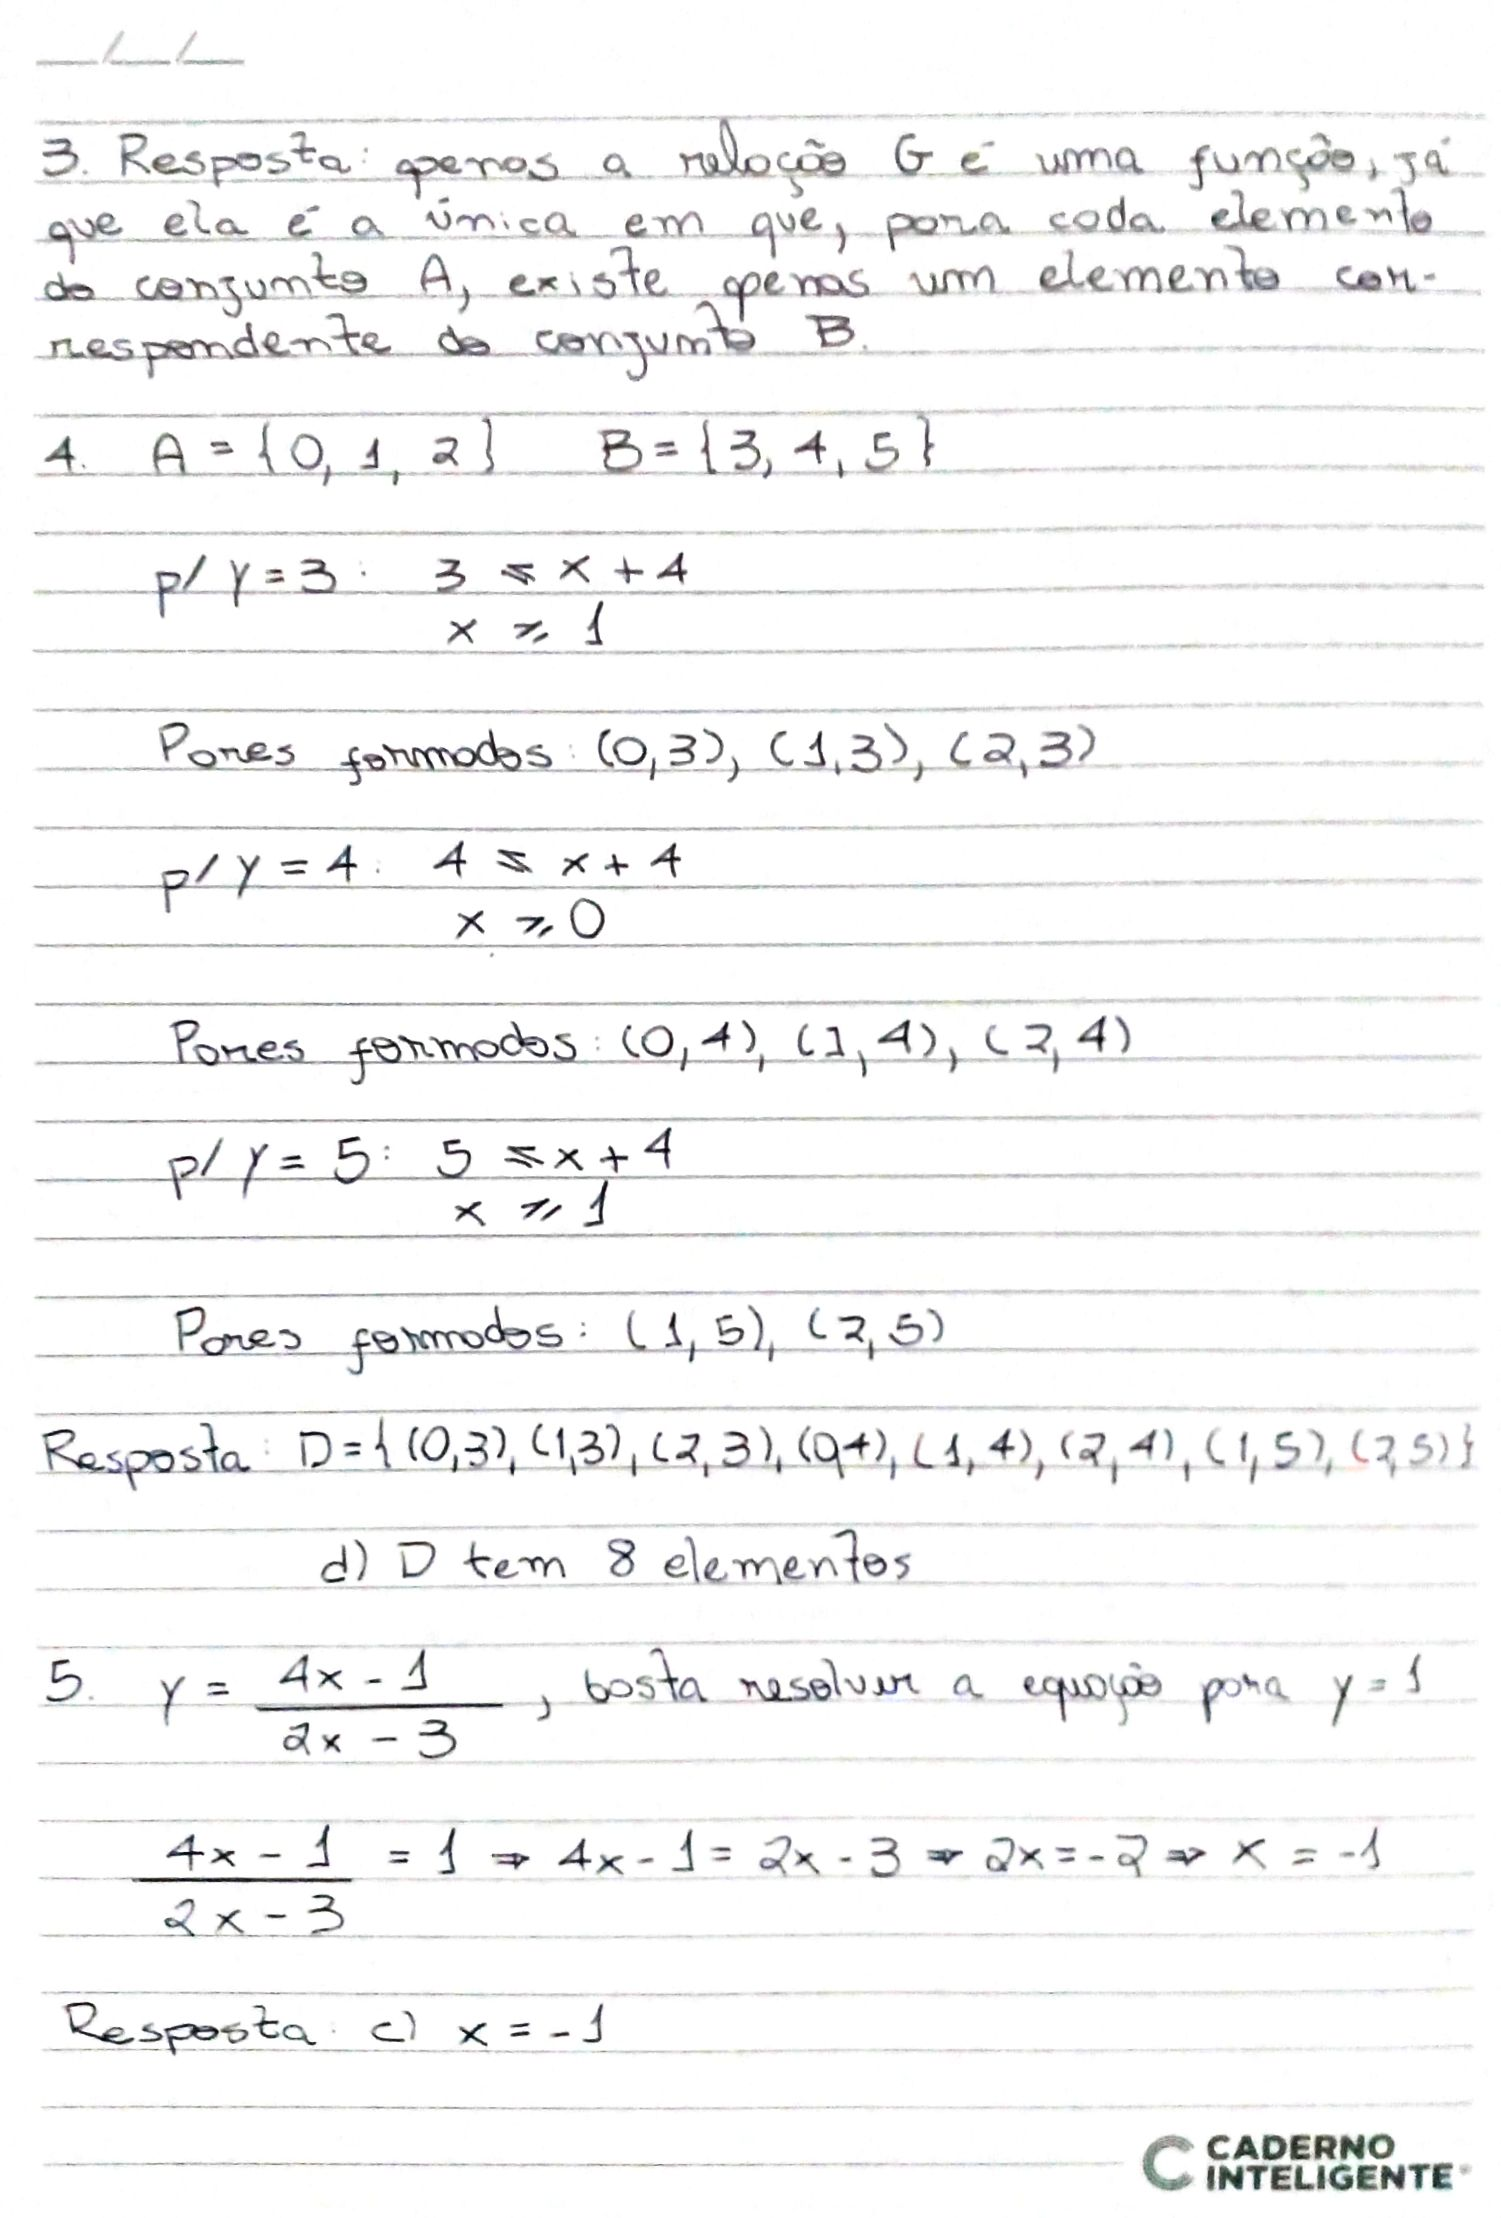
\includegraphics[scale=0.23]{pagina3.jpg}
\end{figure}

\begin{figure}[H]
  \centering
  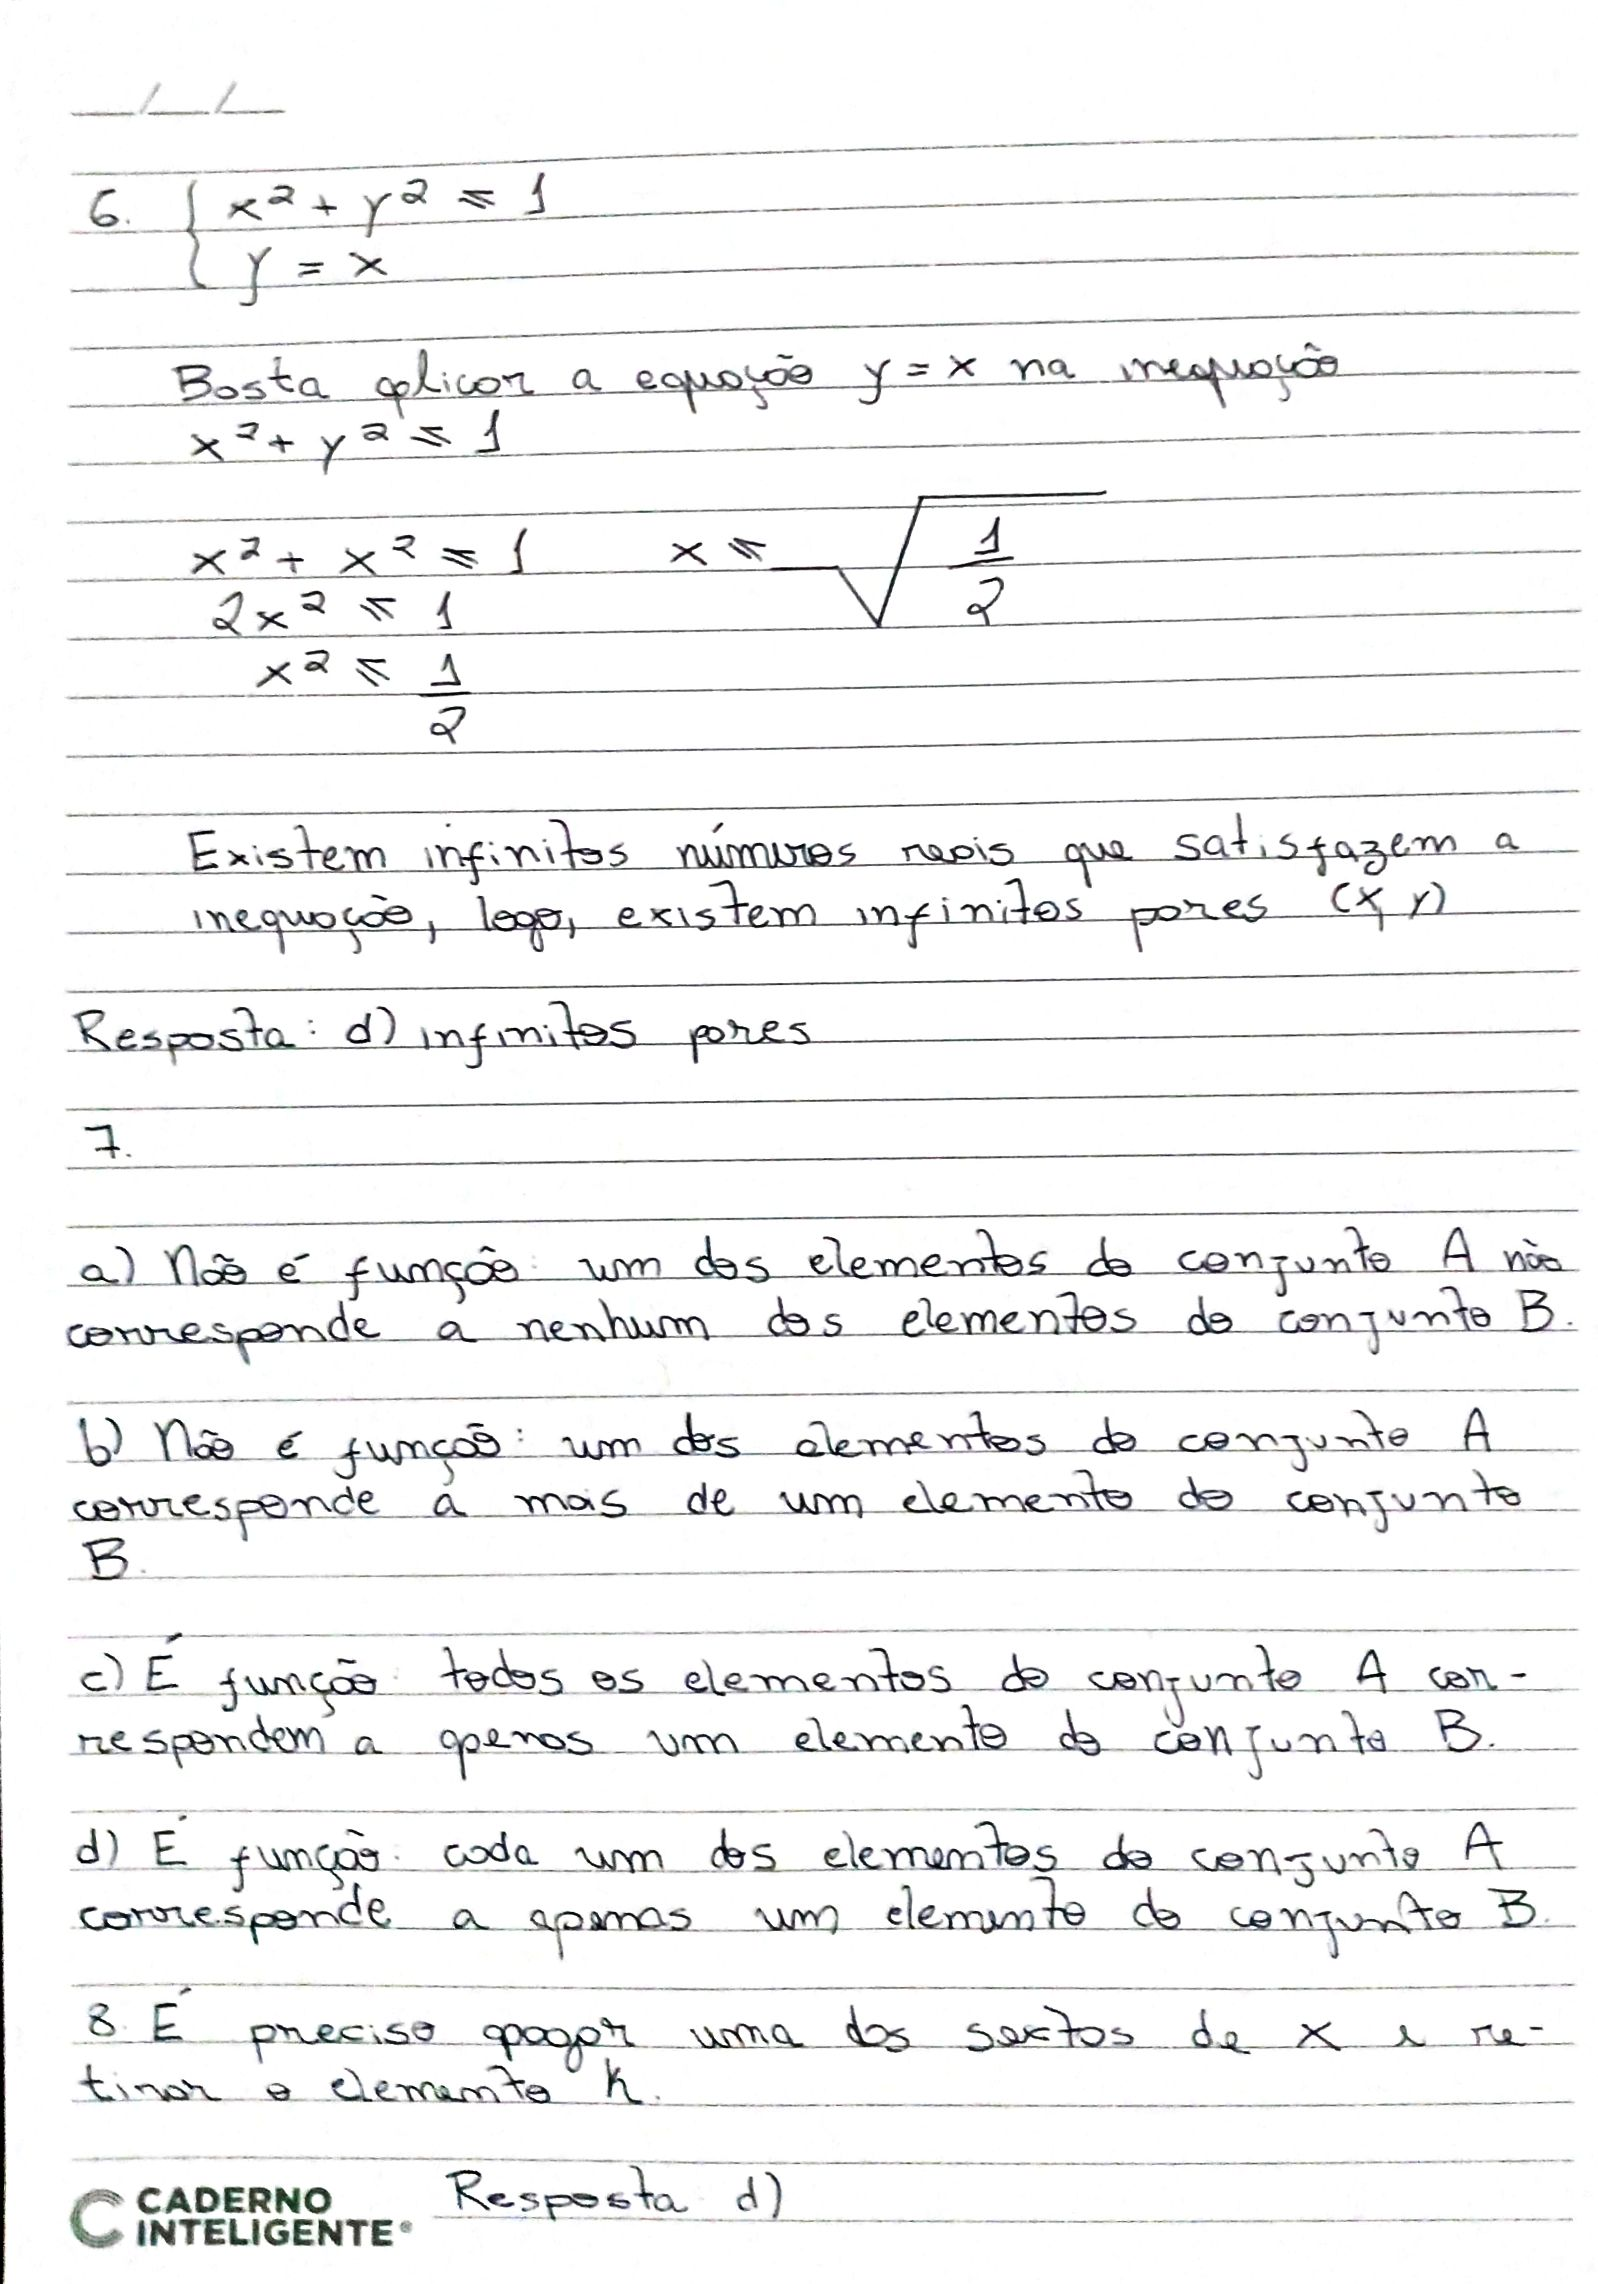
\includegraphics[scale=0.23]{pagina4.jpg}
\end{figure}

\begin{figure}[H]
  \centering
  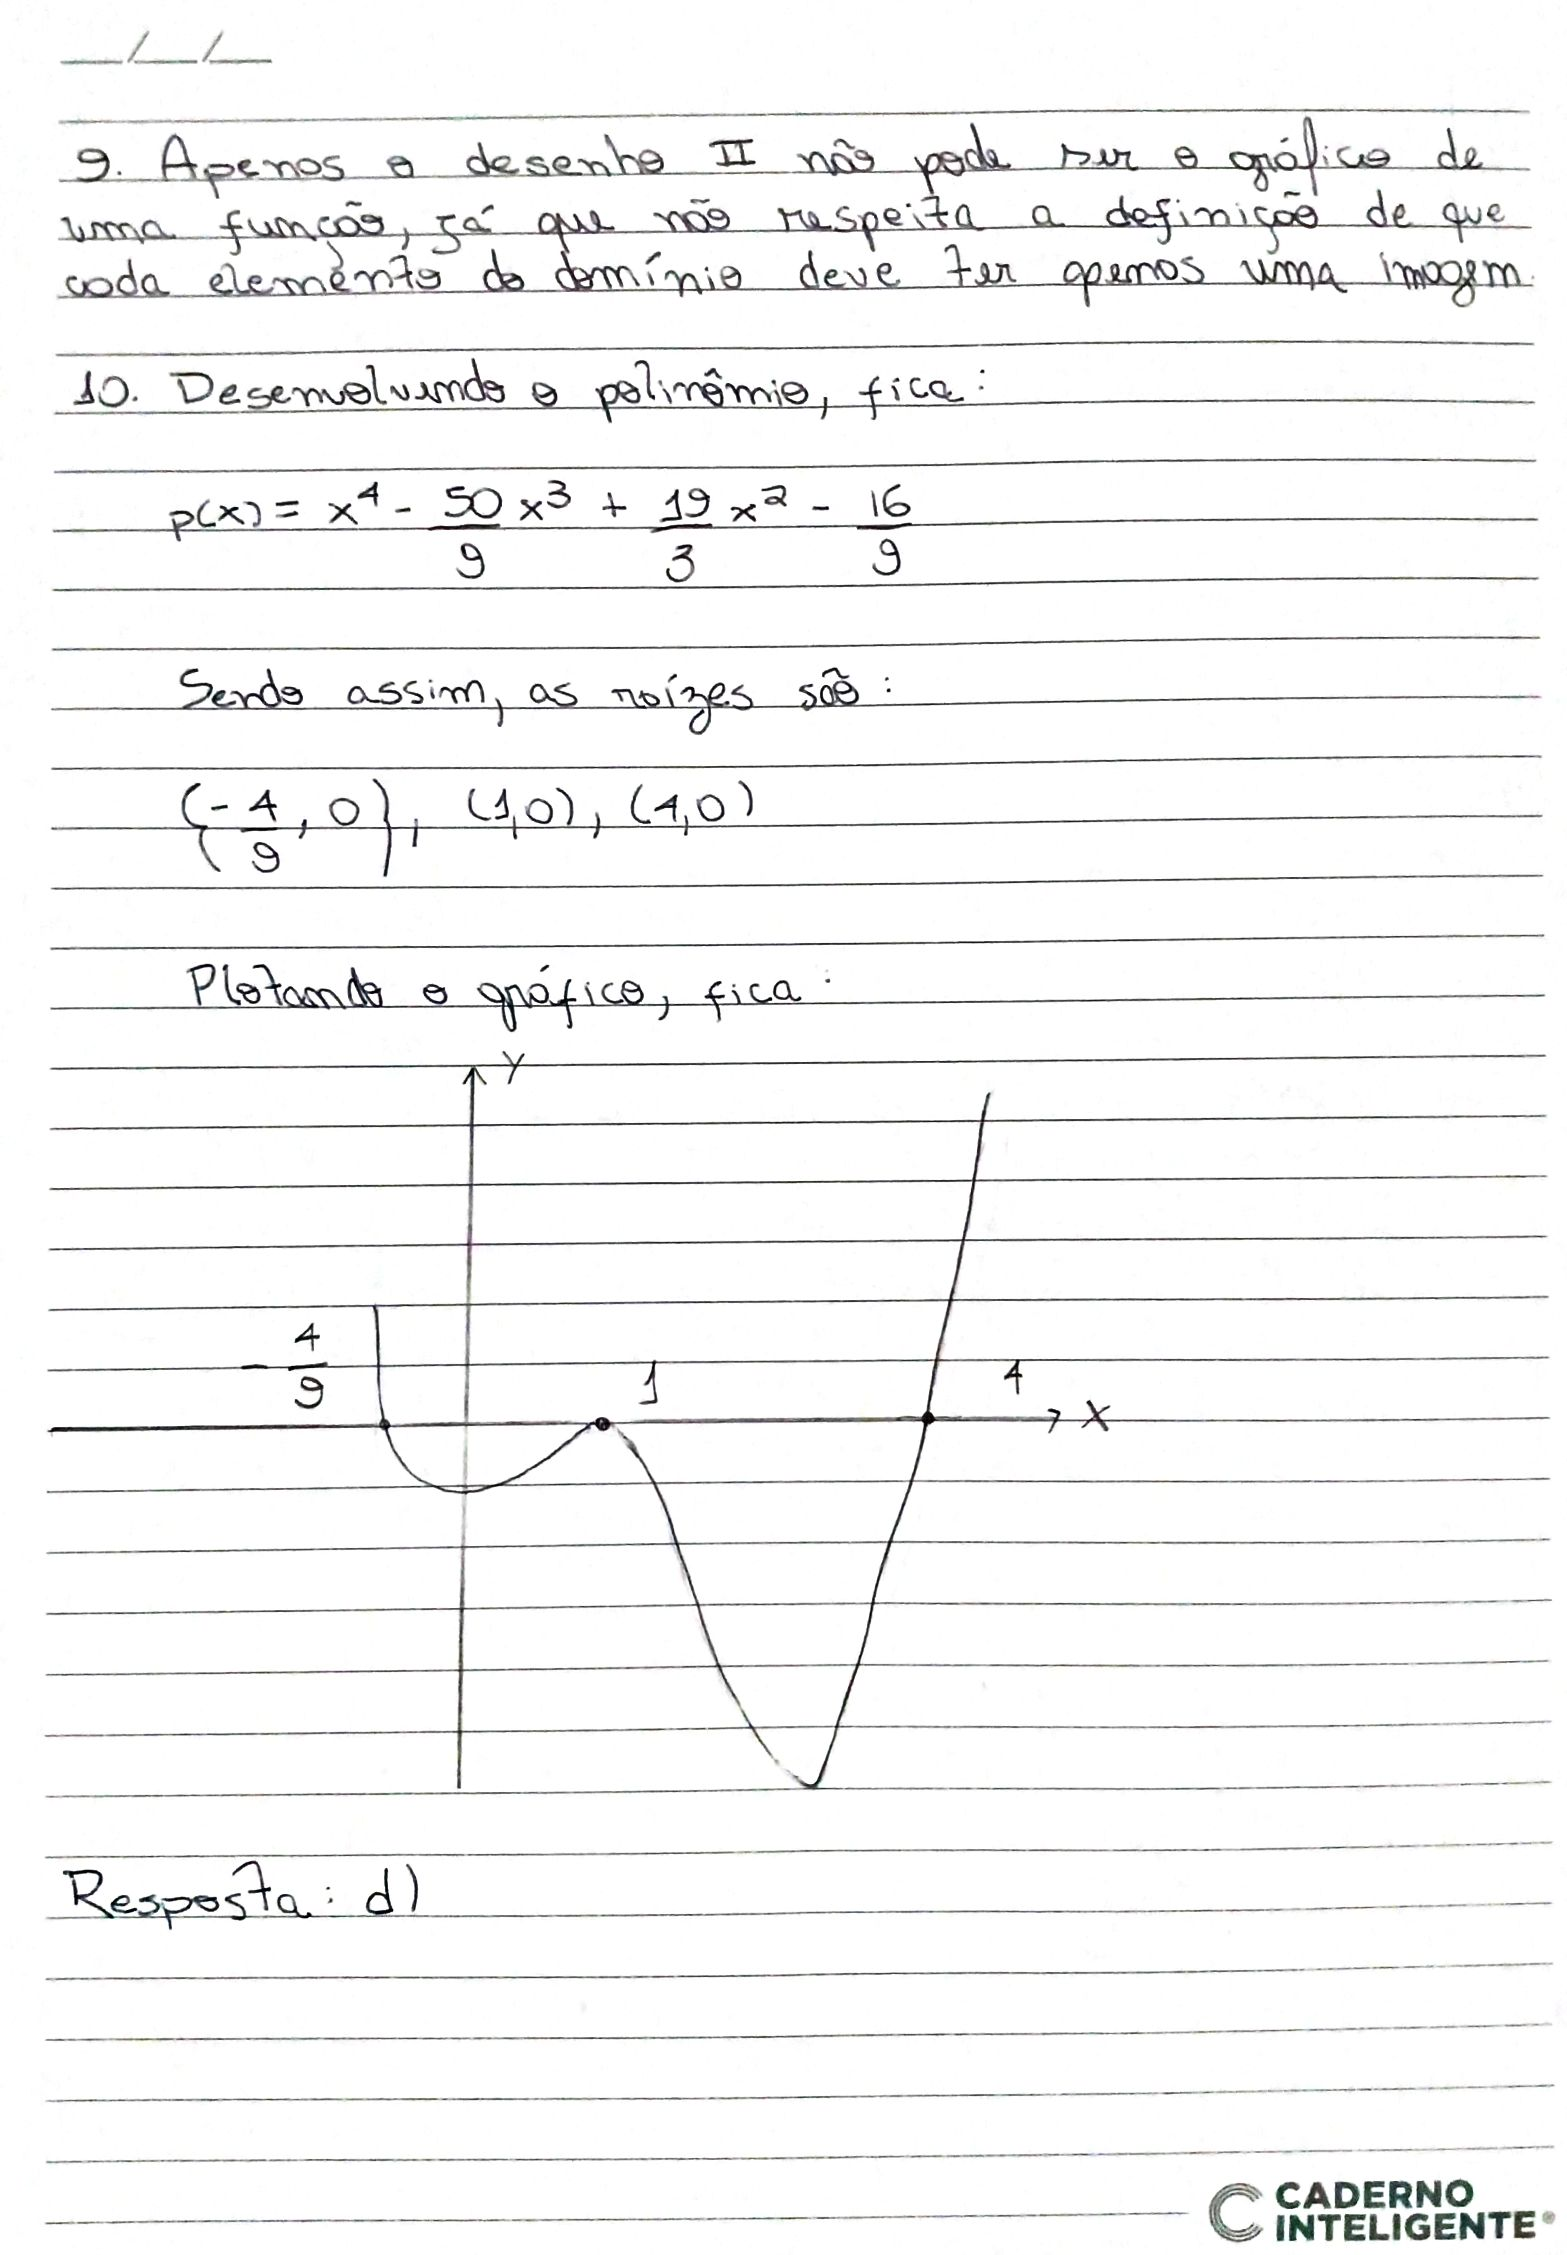
\includegraphics[scale=0.23]{pagina5.jpg}
\end{figure}

\begin{figure}[H]
  \centering
  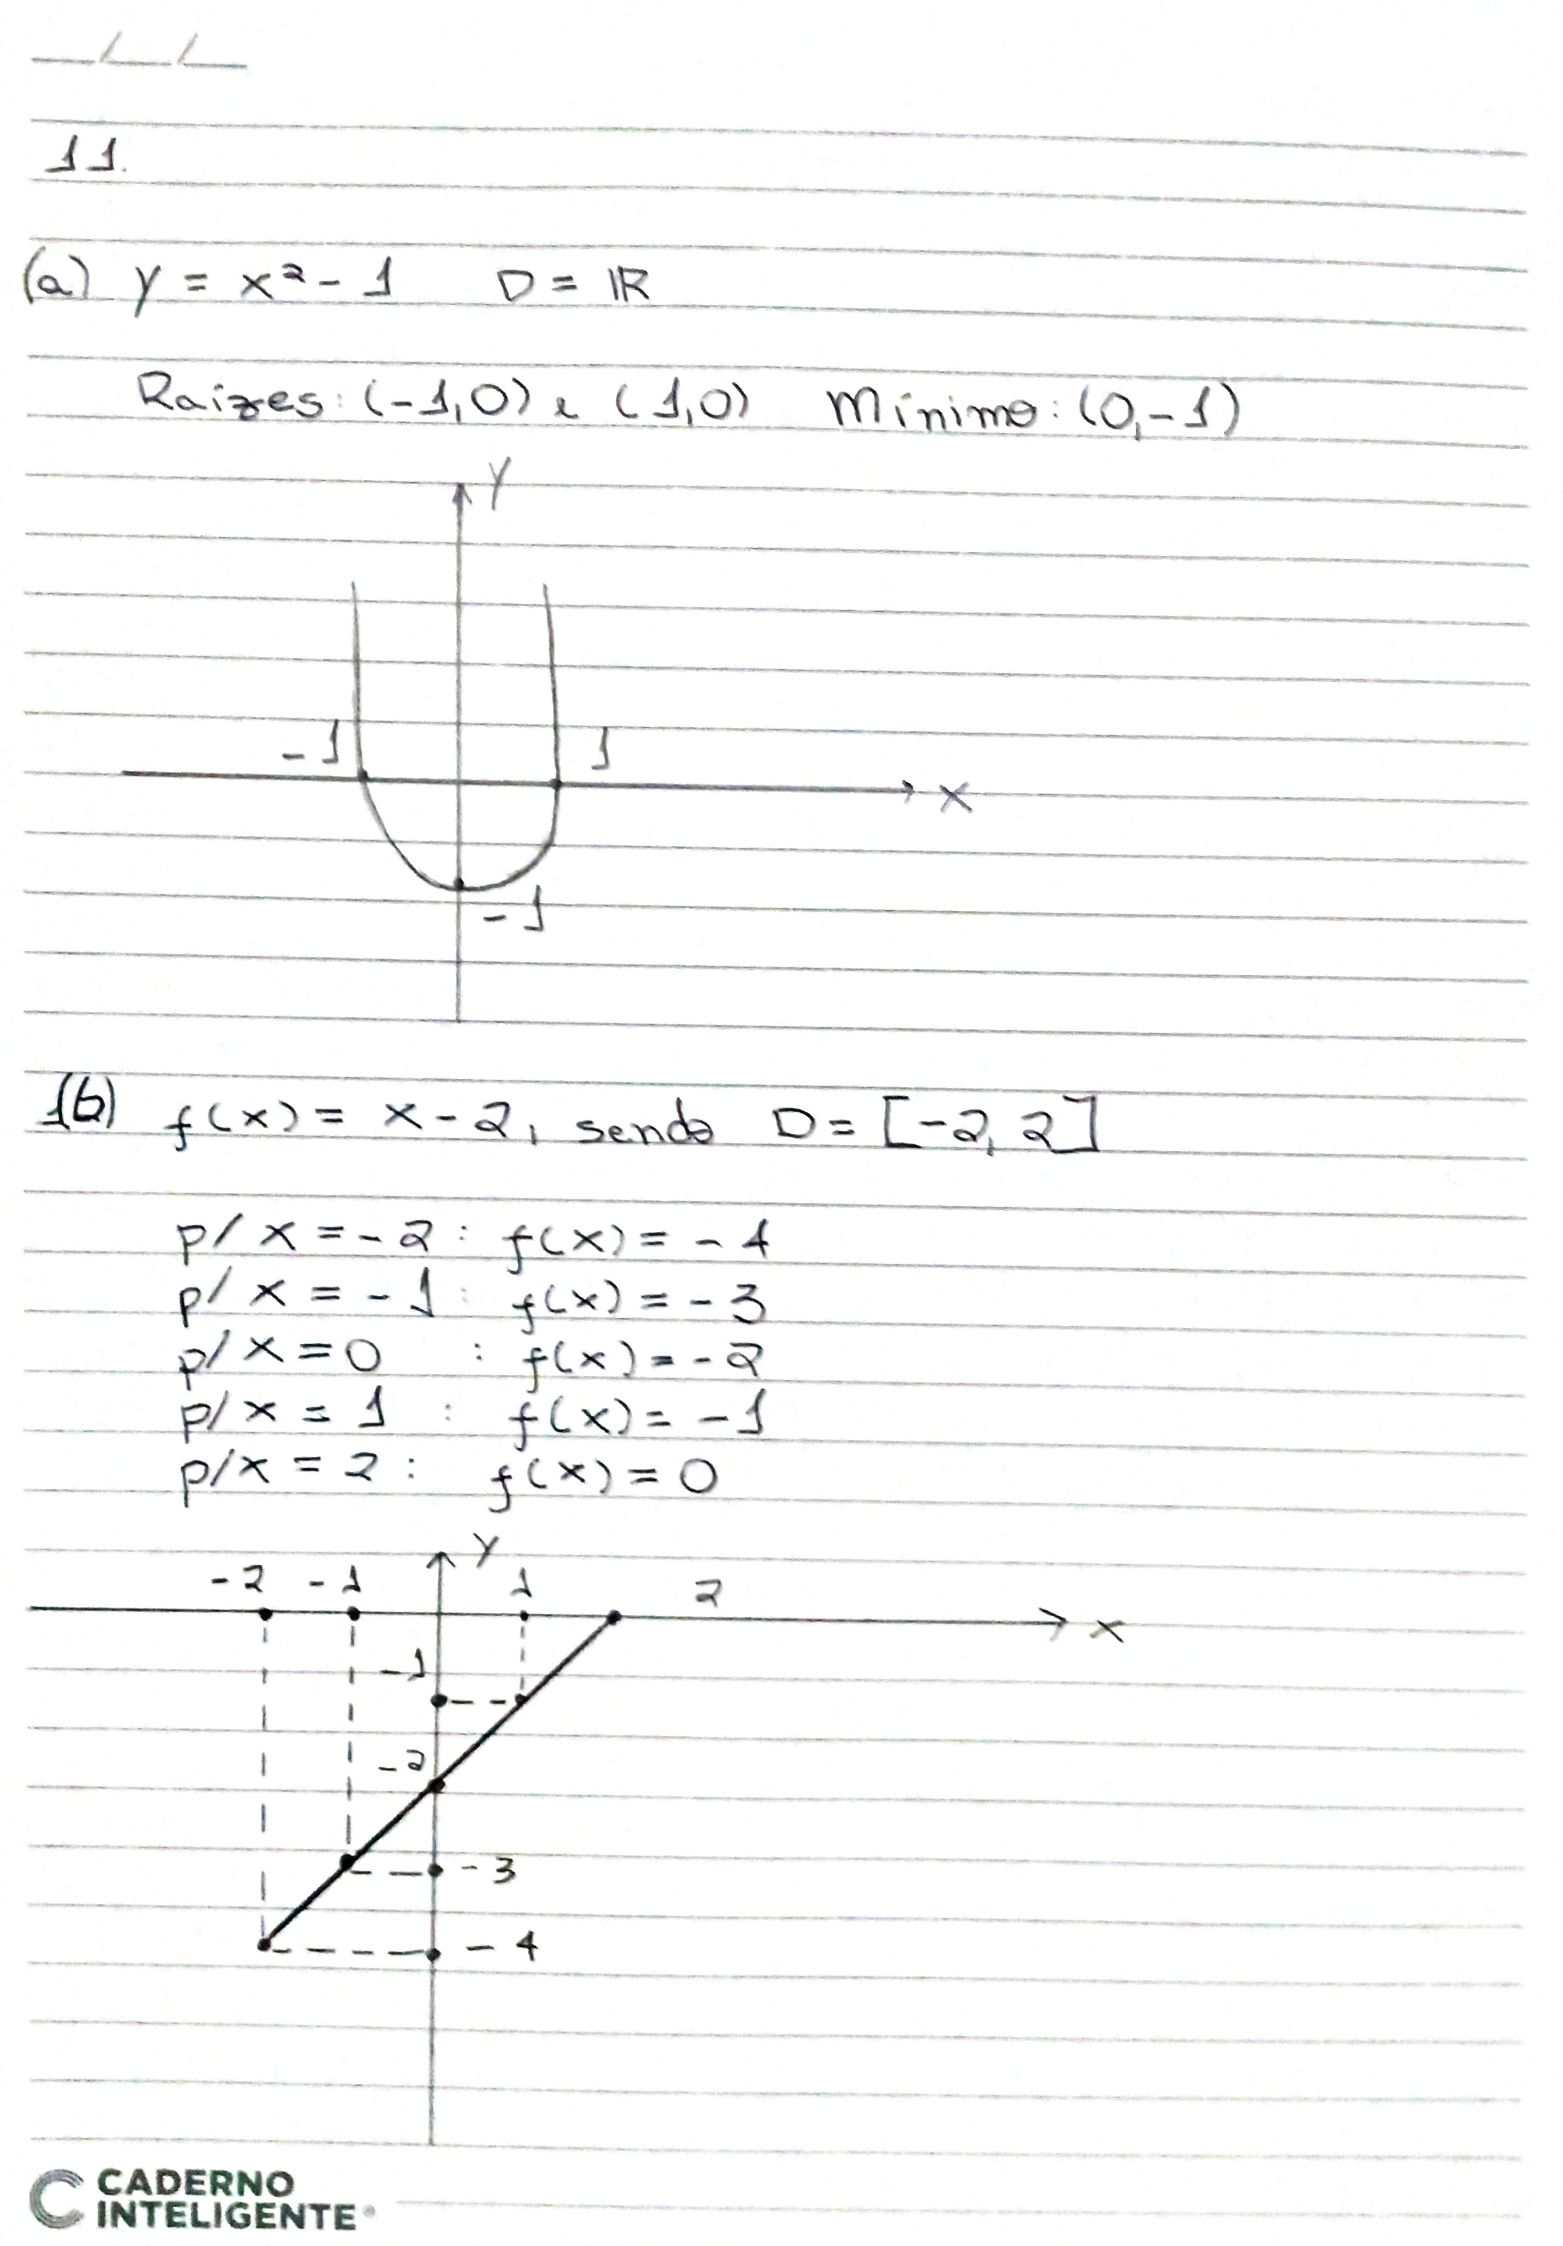
\includegraphics[scale=0.23]{pagina6.jpg}
\end{figure}

\begin{figure}[H]
  \centering
  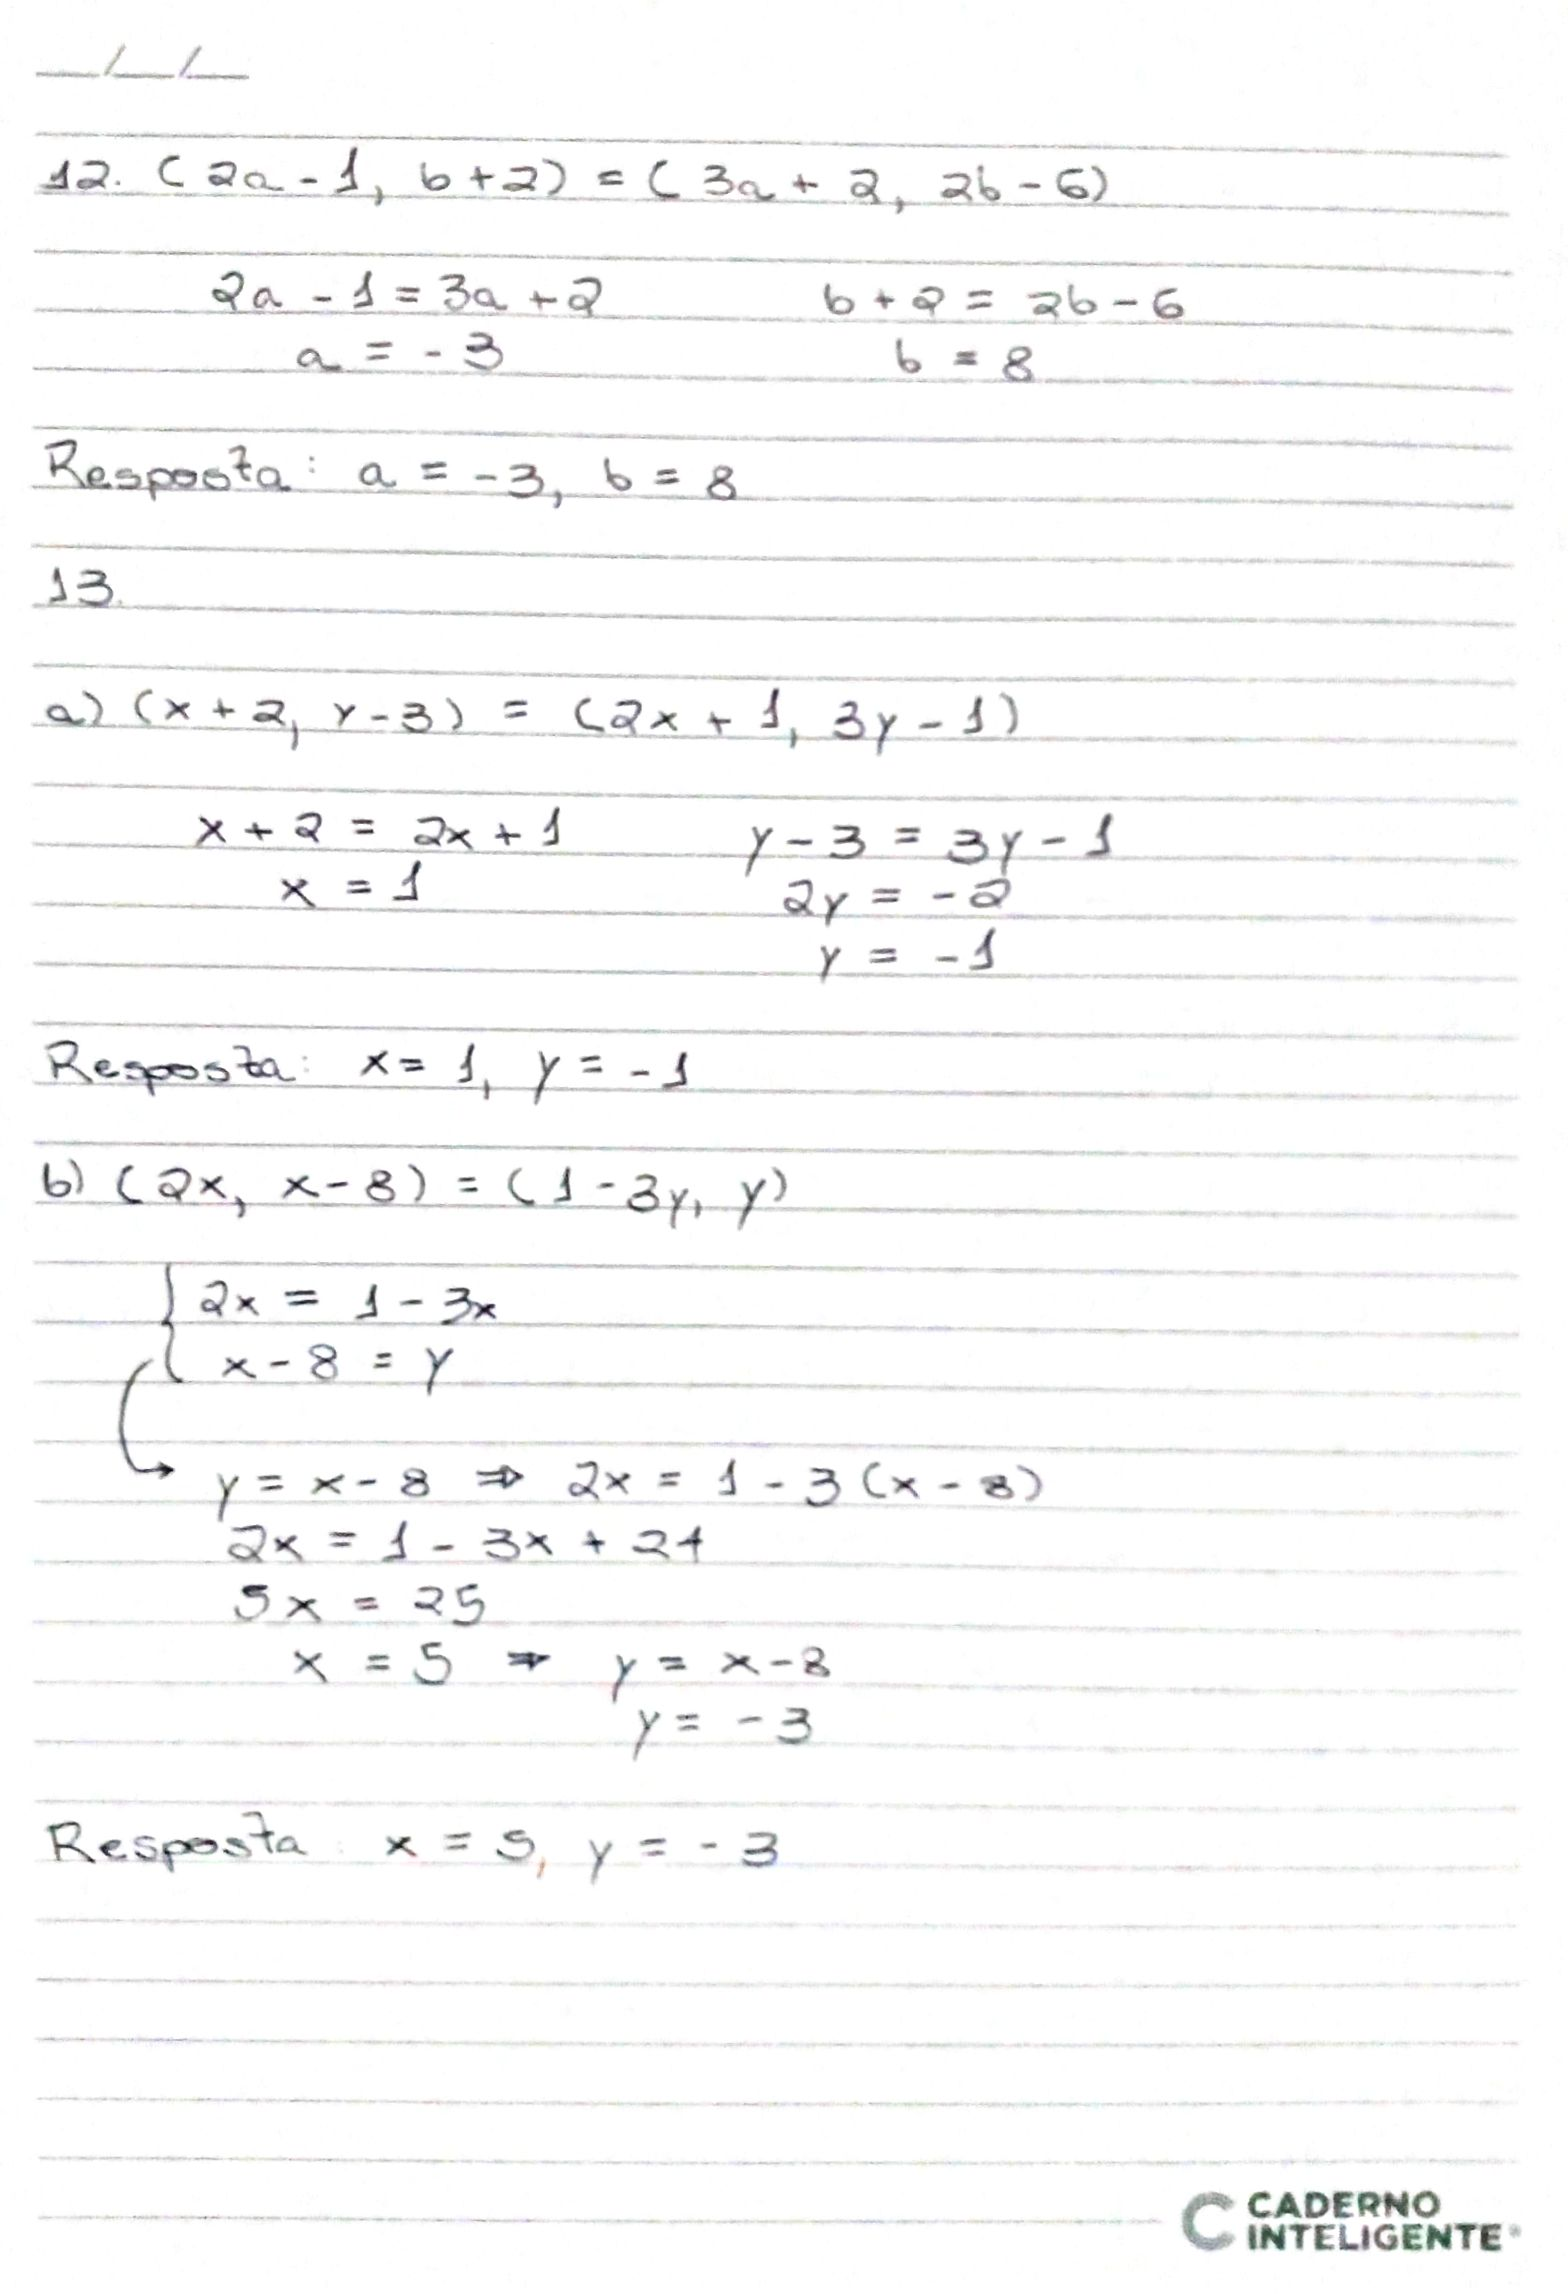
\includegraphics[scale=0.23]{pagina7.jpg}
\end{figure}

\begin{figure}[H]
  \centering
  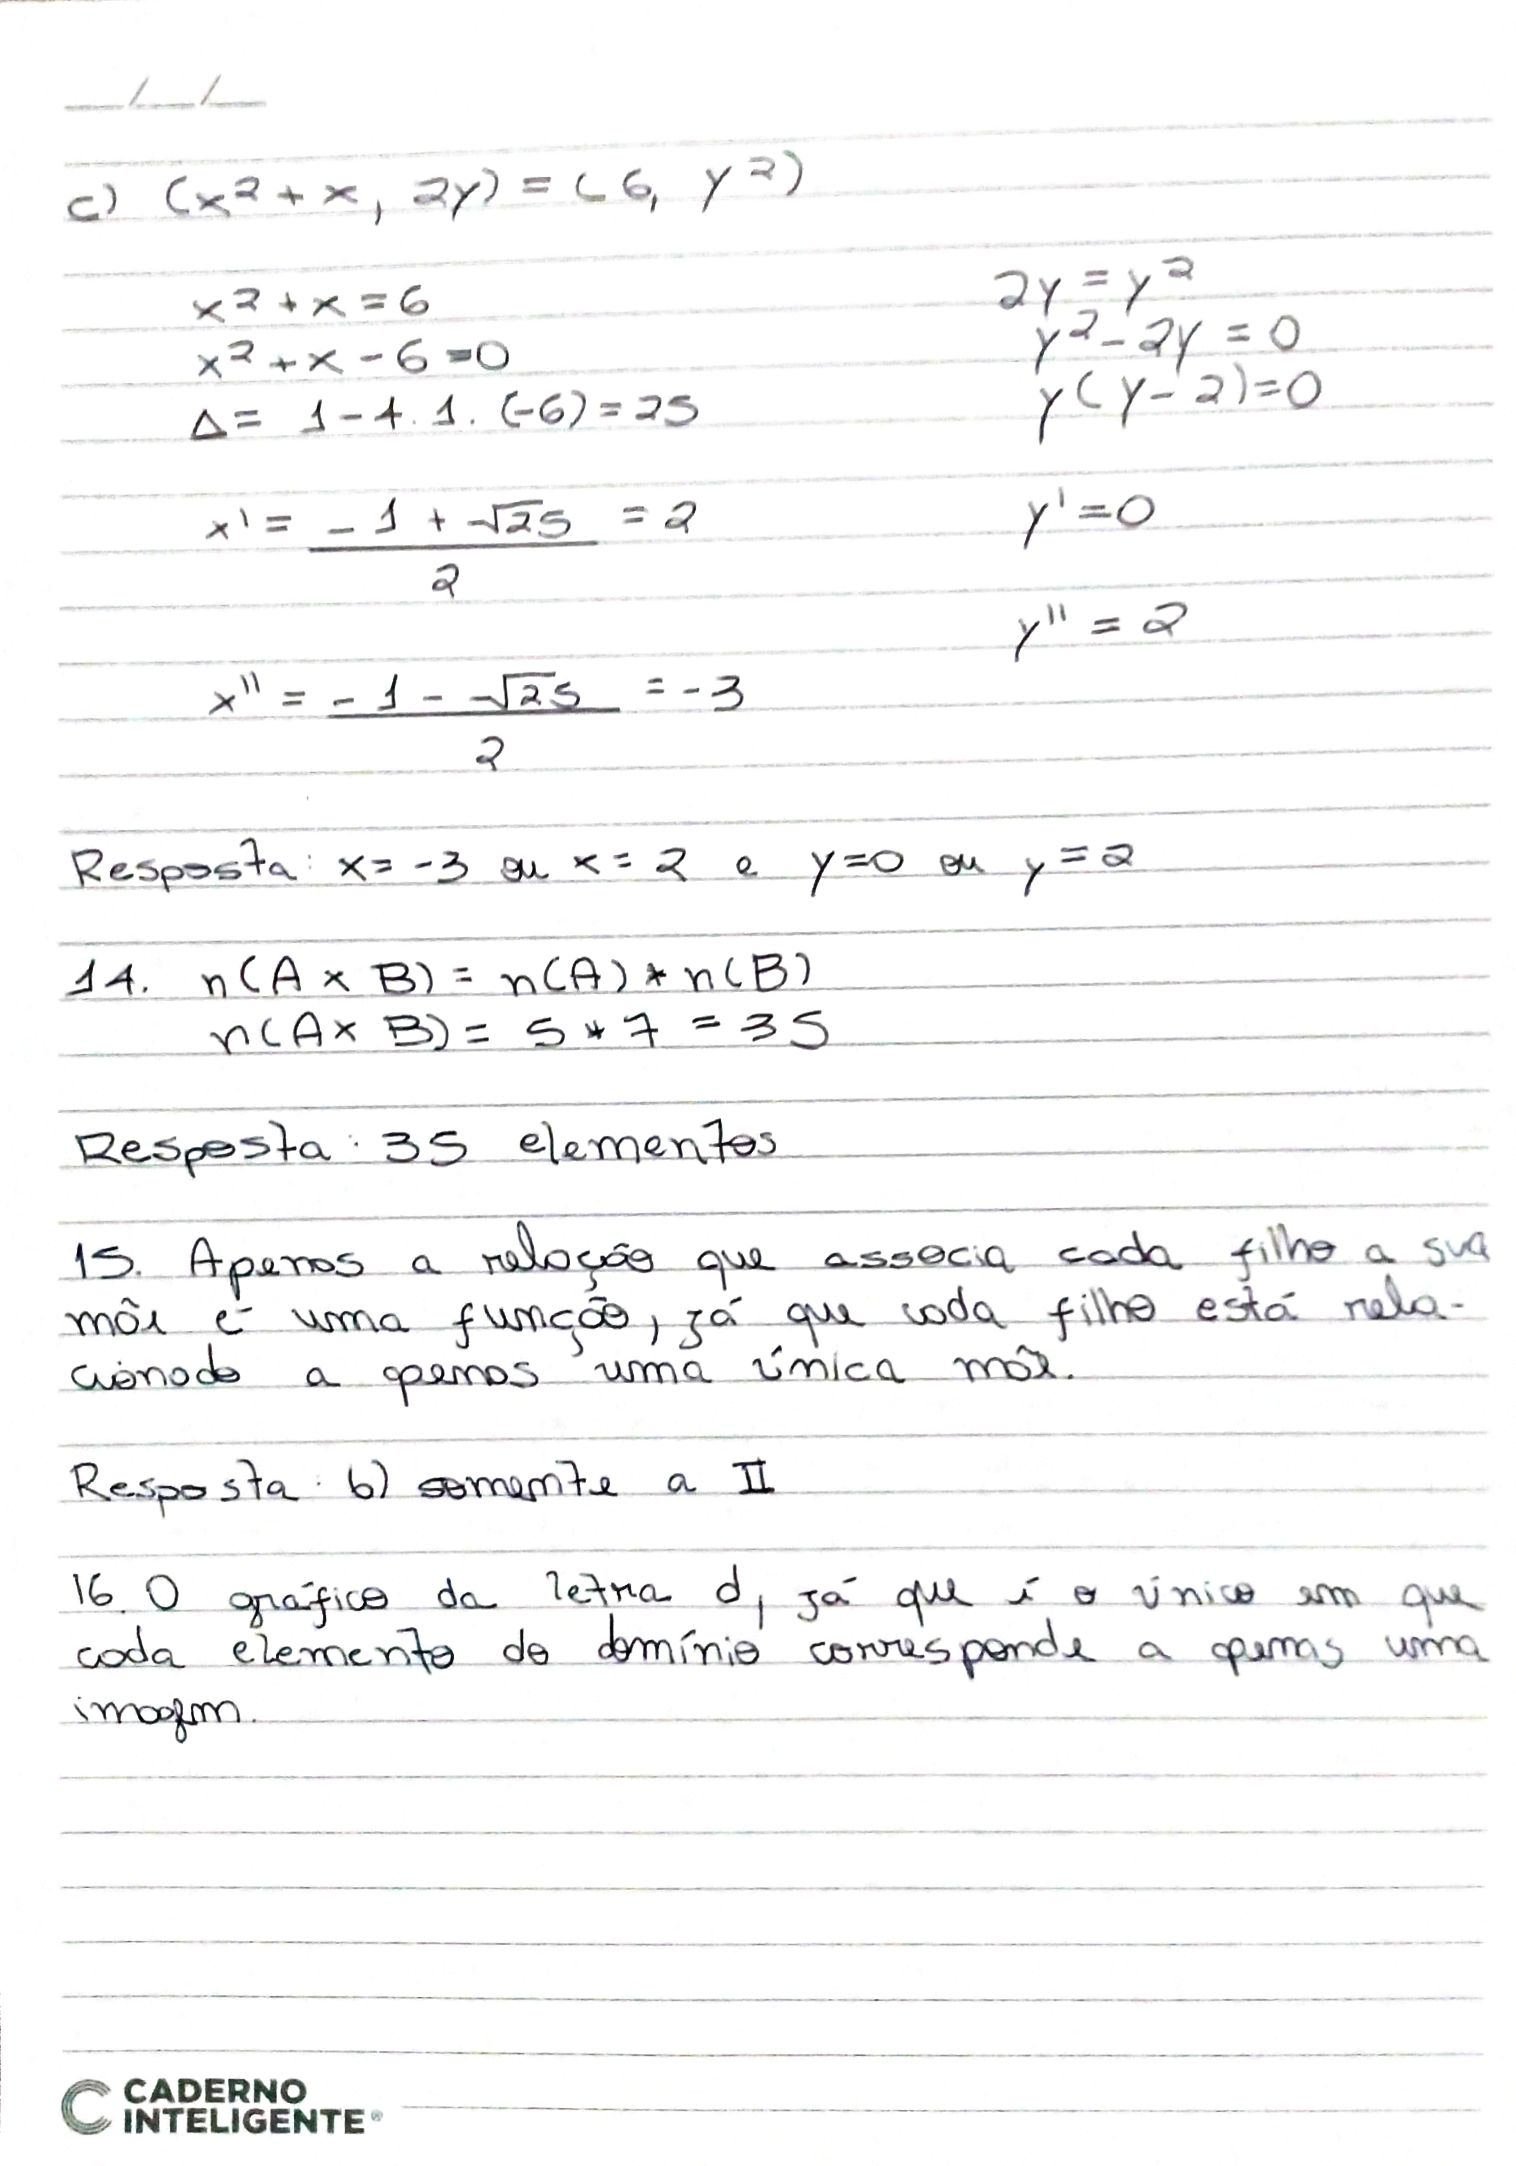
\includegraphics[scale=0.23]{pagina8.jpg}
\end{figure}

\begin{figure}[H]
  \centering
  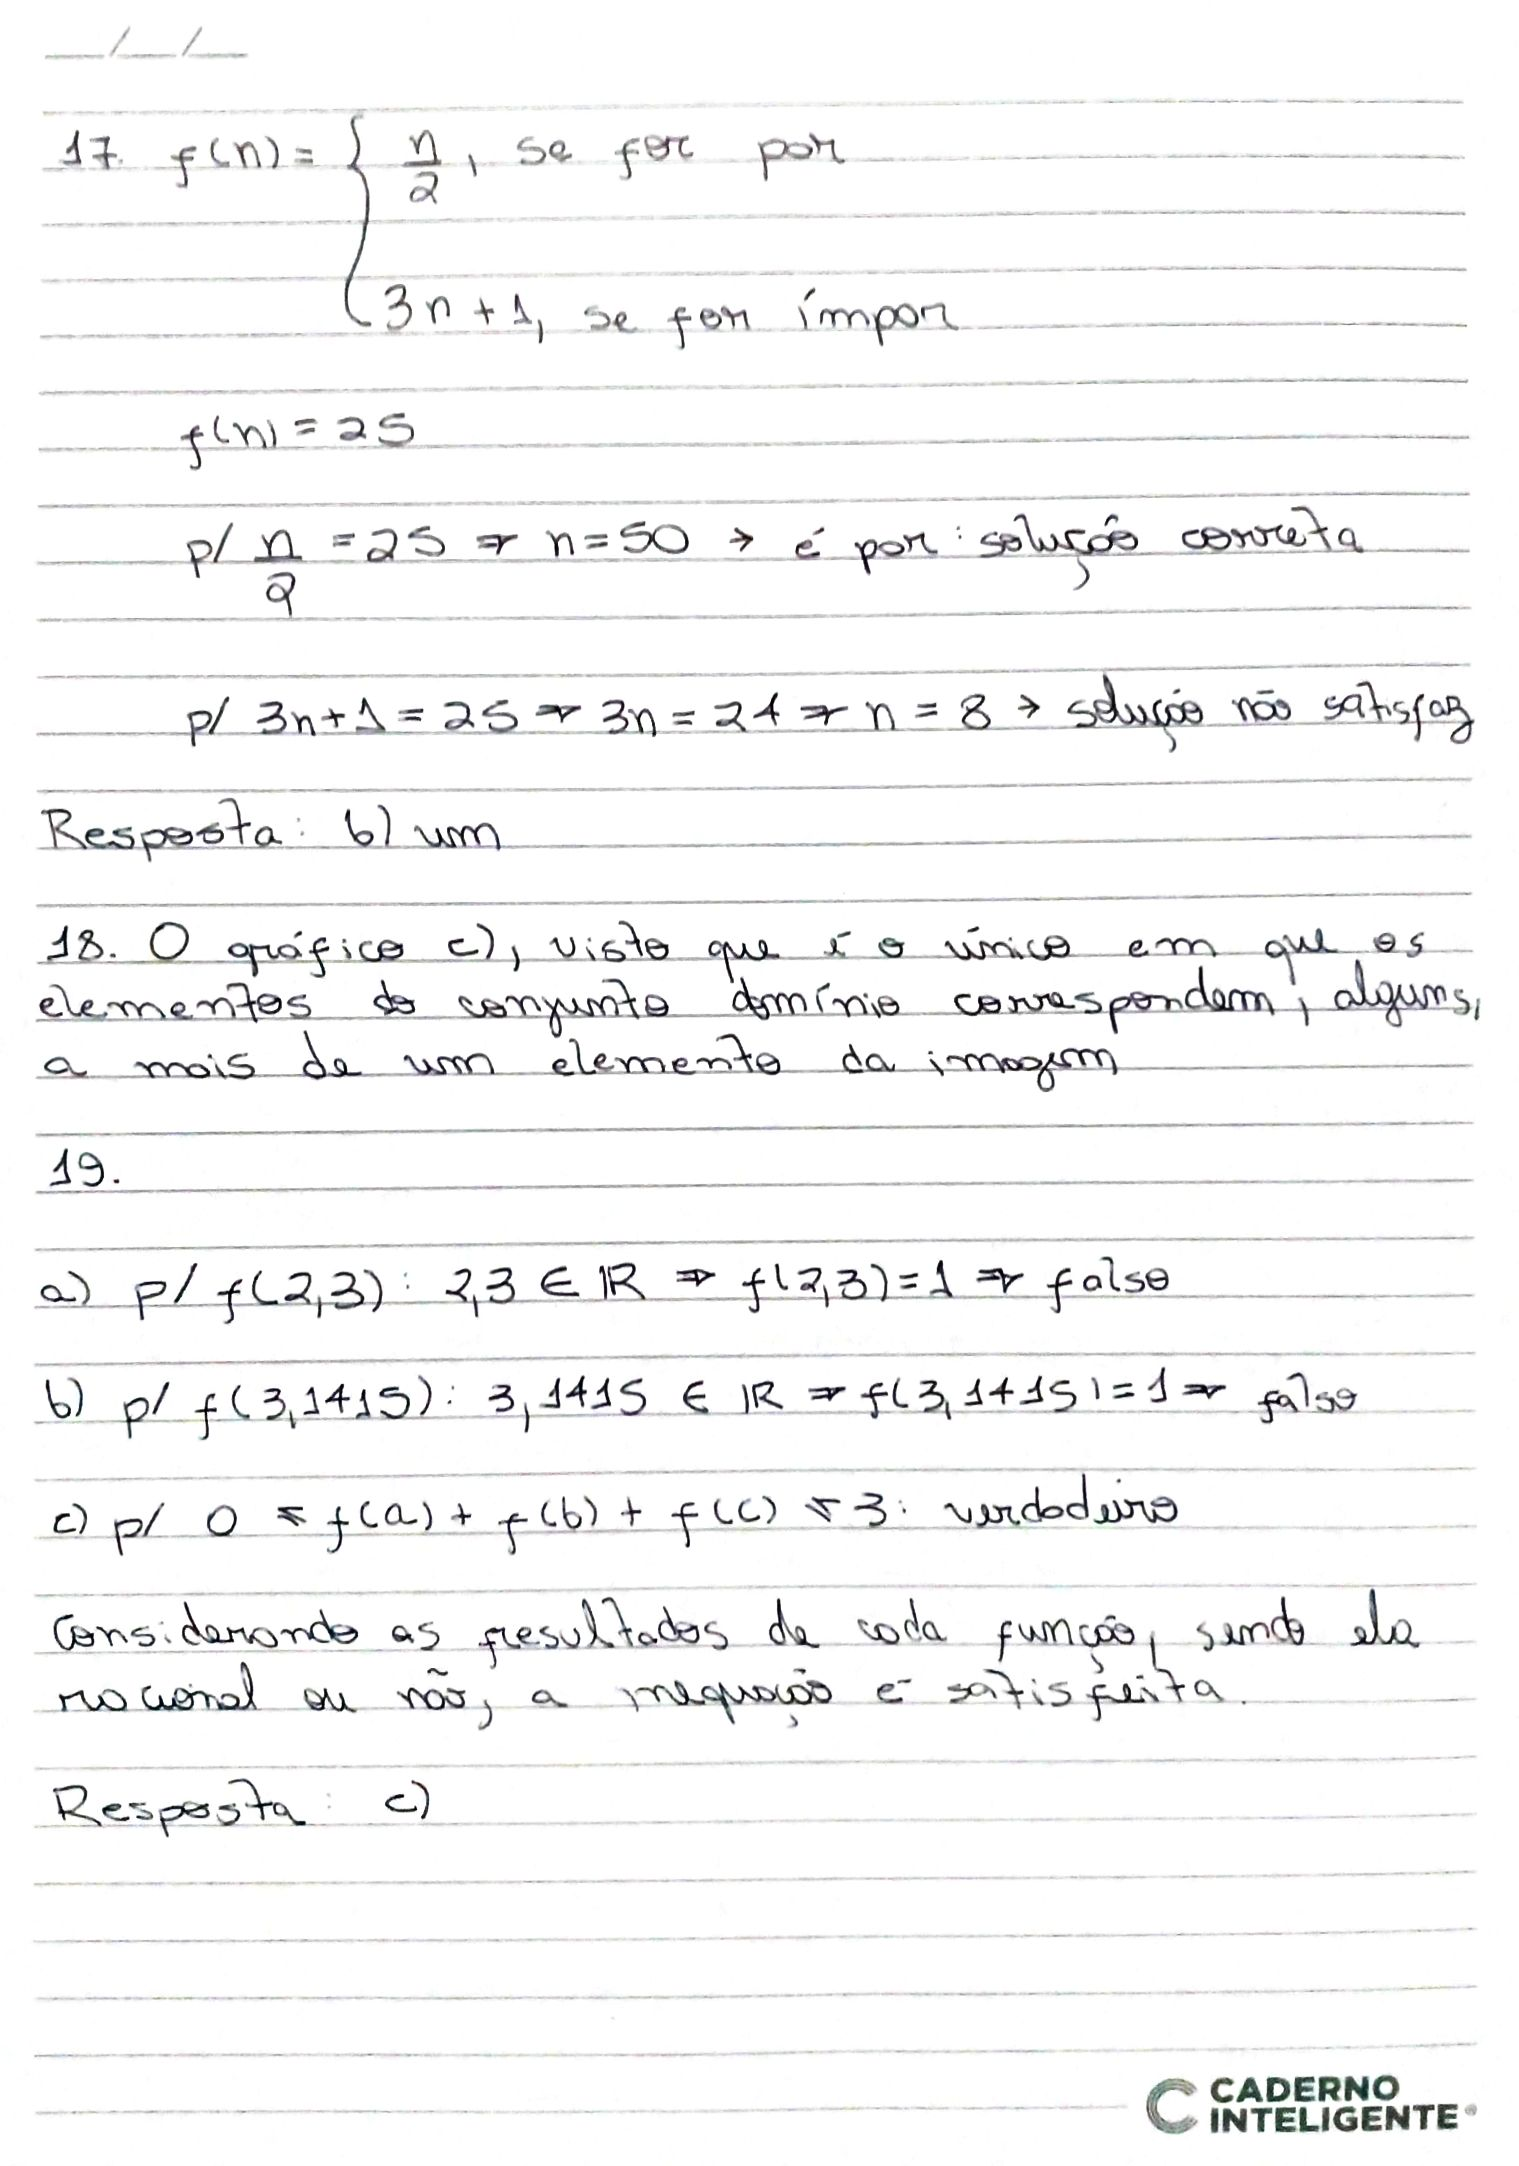
\includegraphics[scale=0.23]{pagina9.jpg}
\end{figure}

\begin{figure}[H]
  \centering
  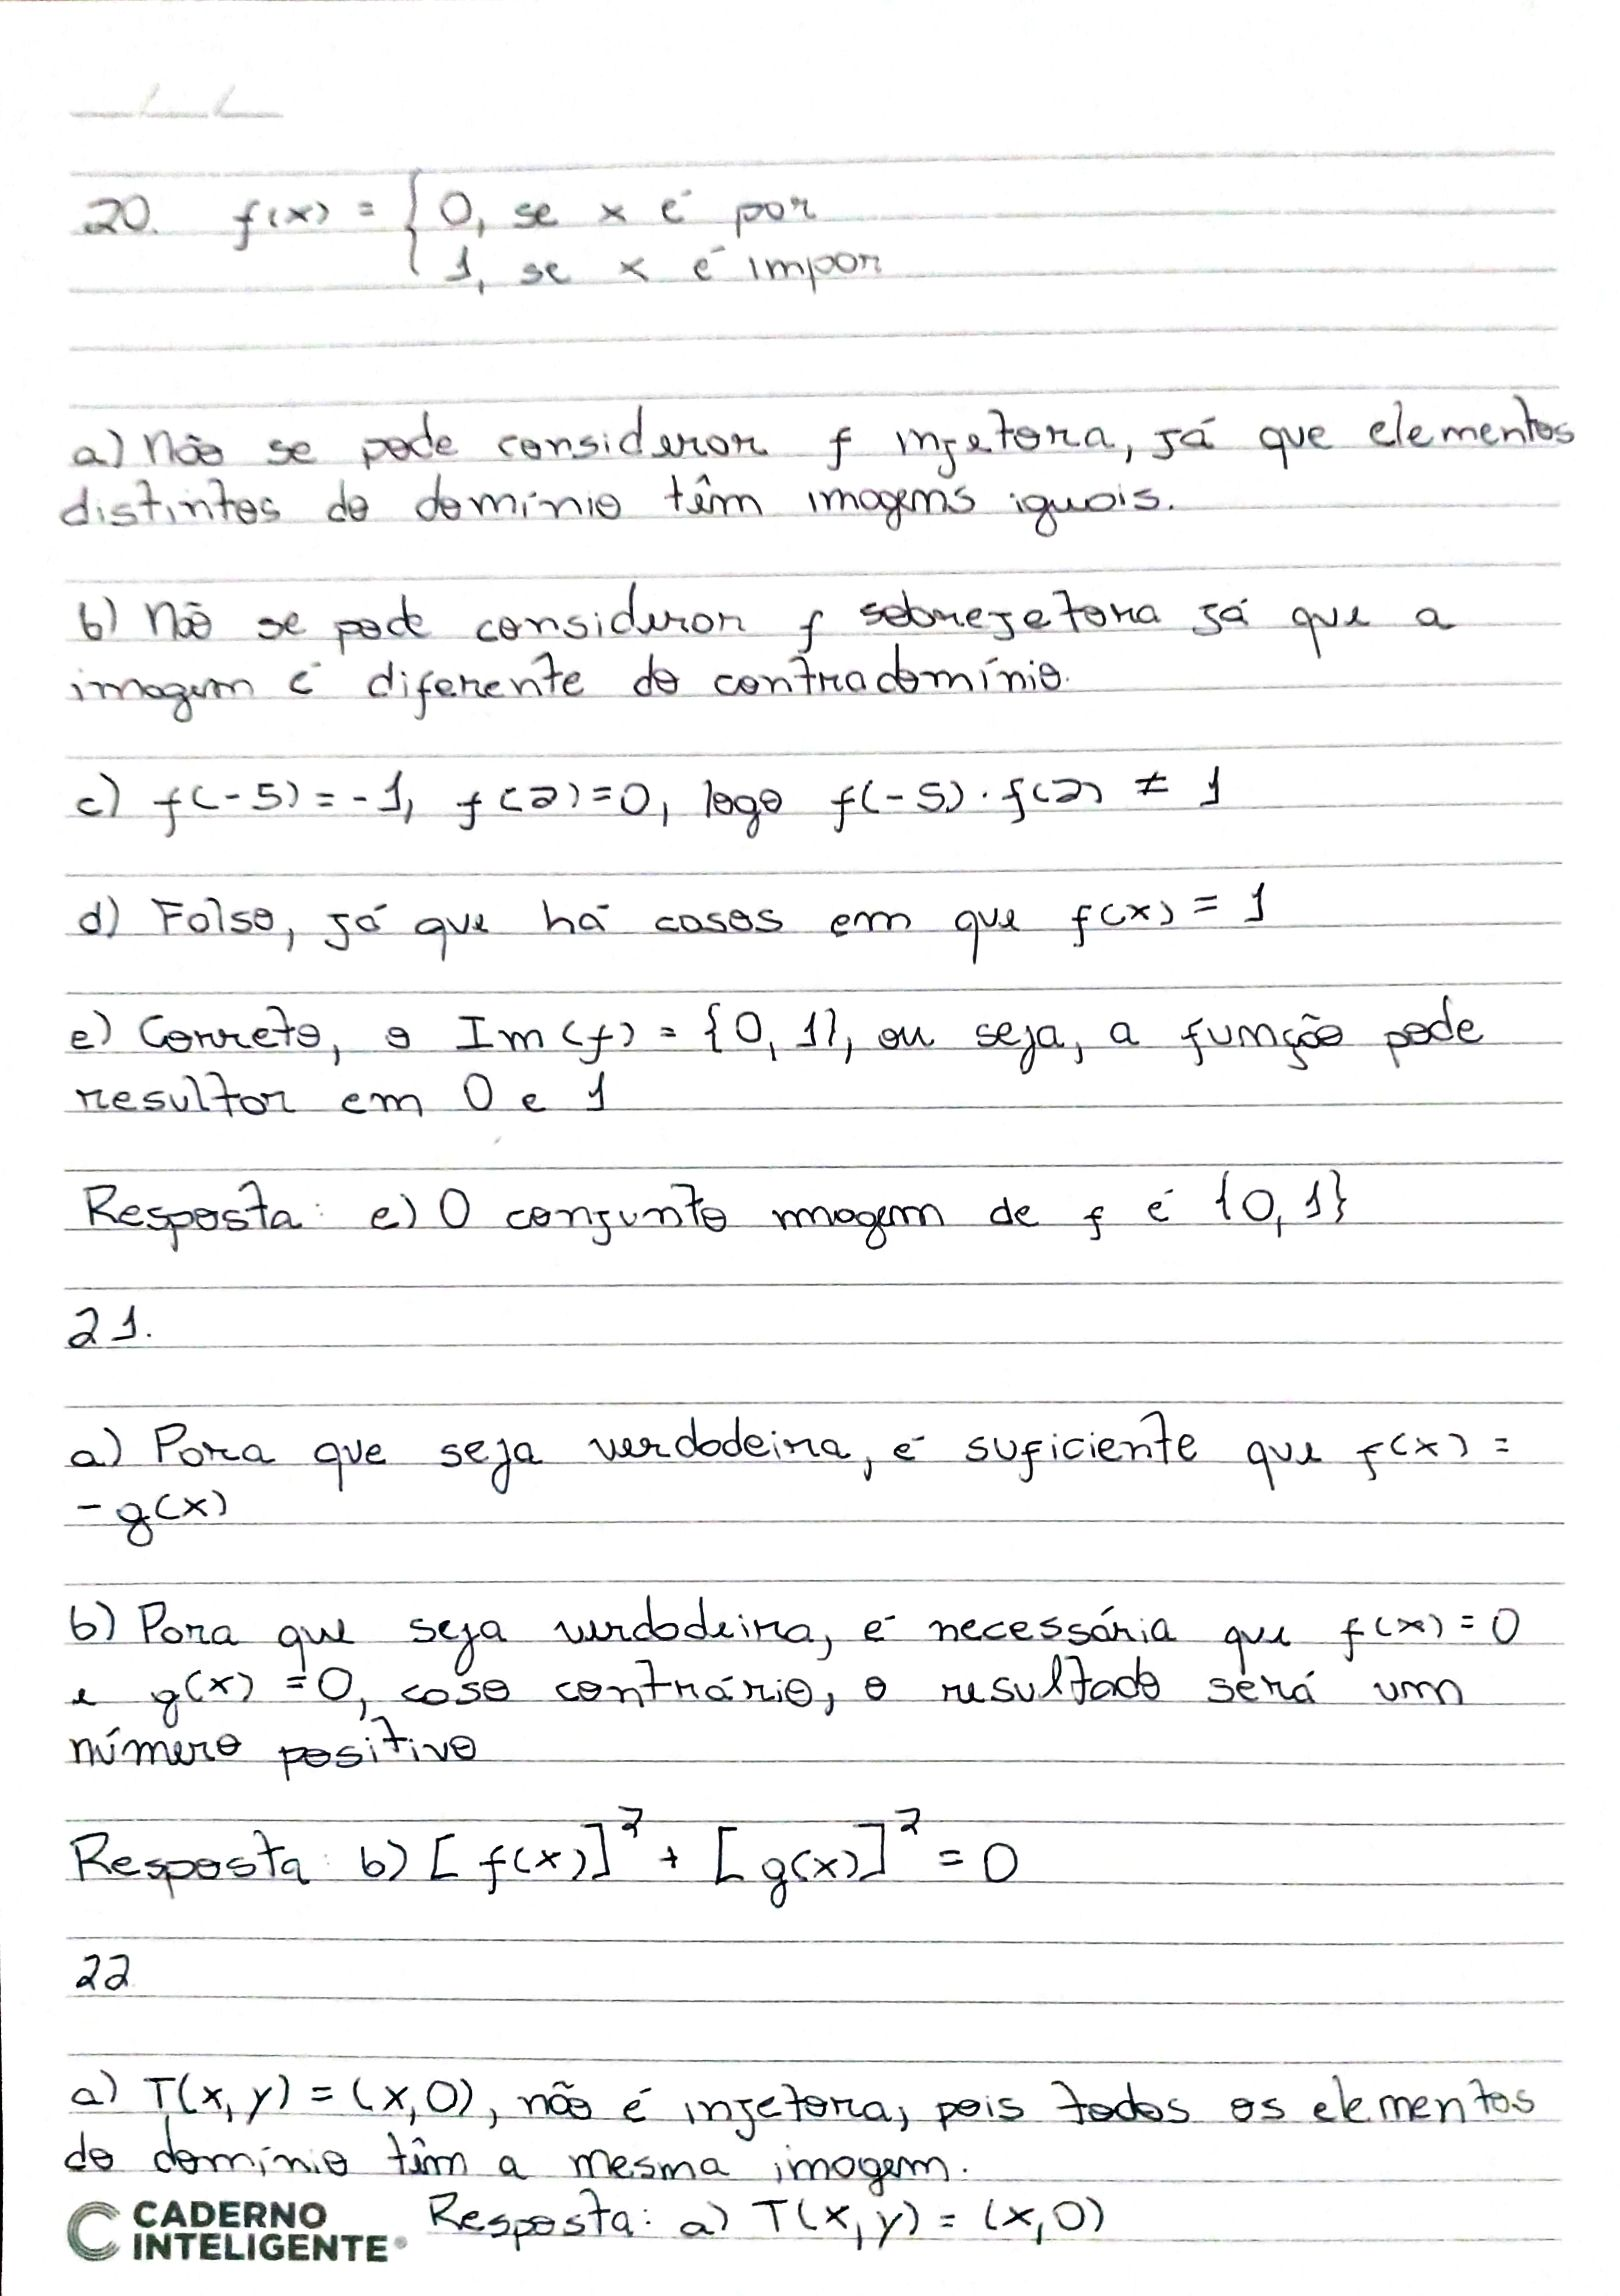
\includegraphics[scale=0.23]{pagina10.jpg}
\end{figure}
% ------------------------------------------------------------
% Exercícios da Série B
% ------------------------------------------------------------
\section{Série B}

\begin{figure}[H]
  \centering
  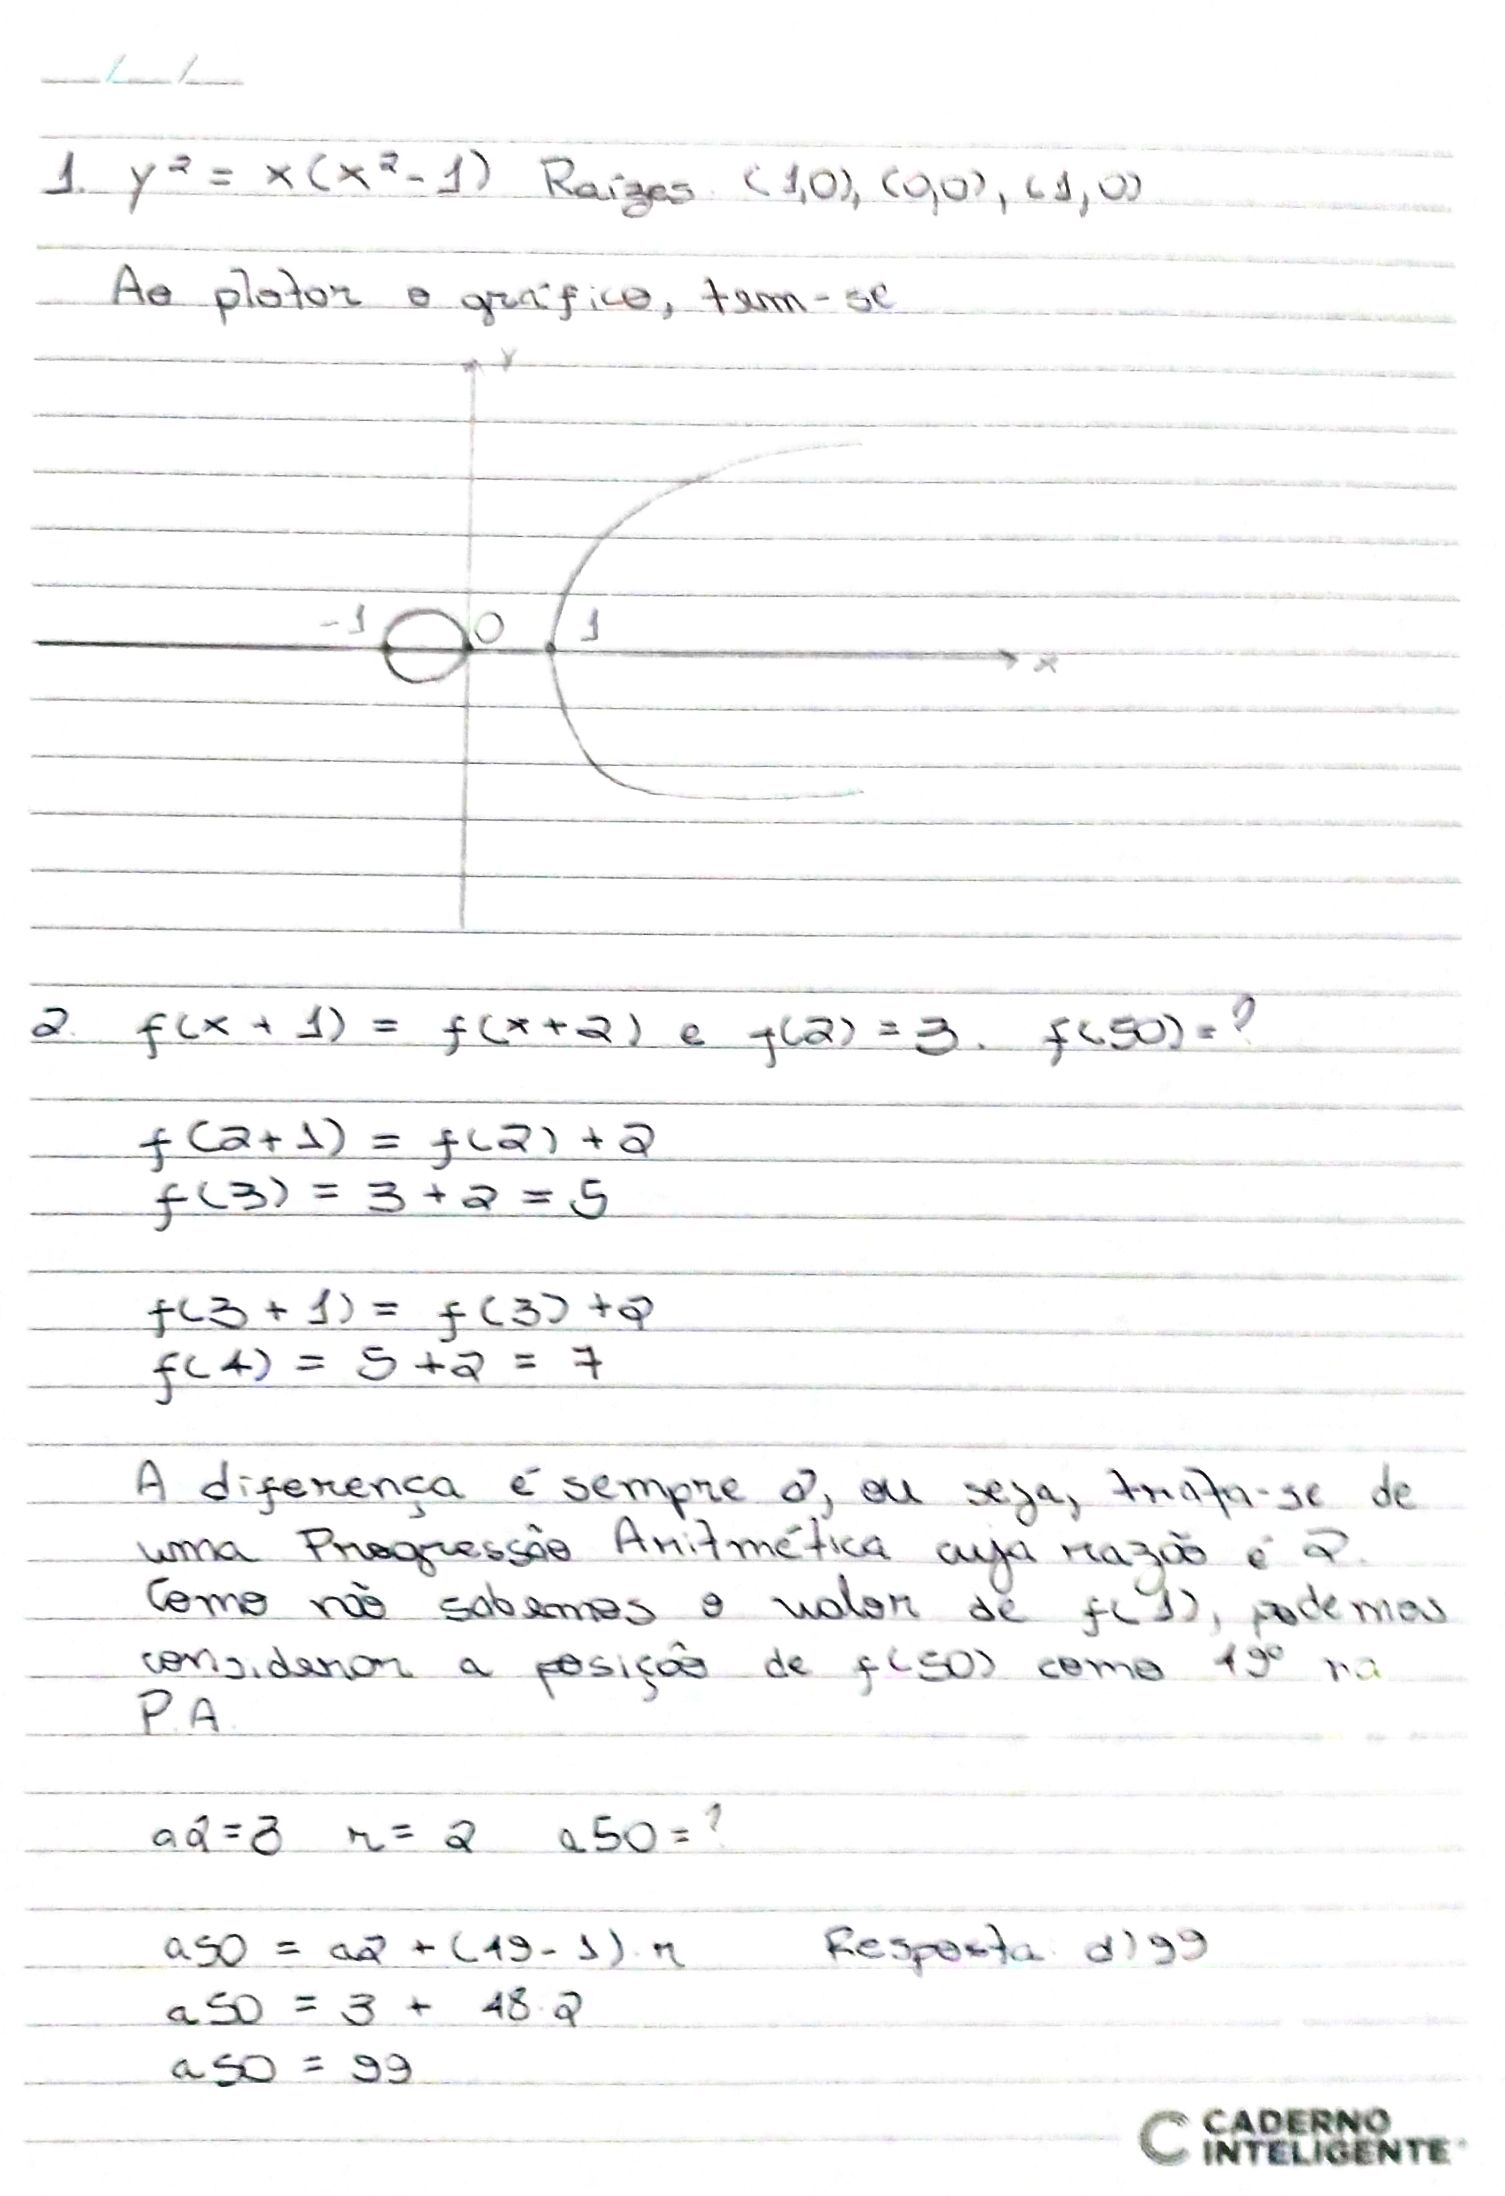
\includegraphics[scale=0.23]{pagina11.jpg}
\end{figure}

\begin{figure}[H]
  \centering
  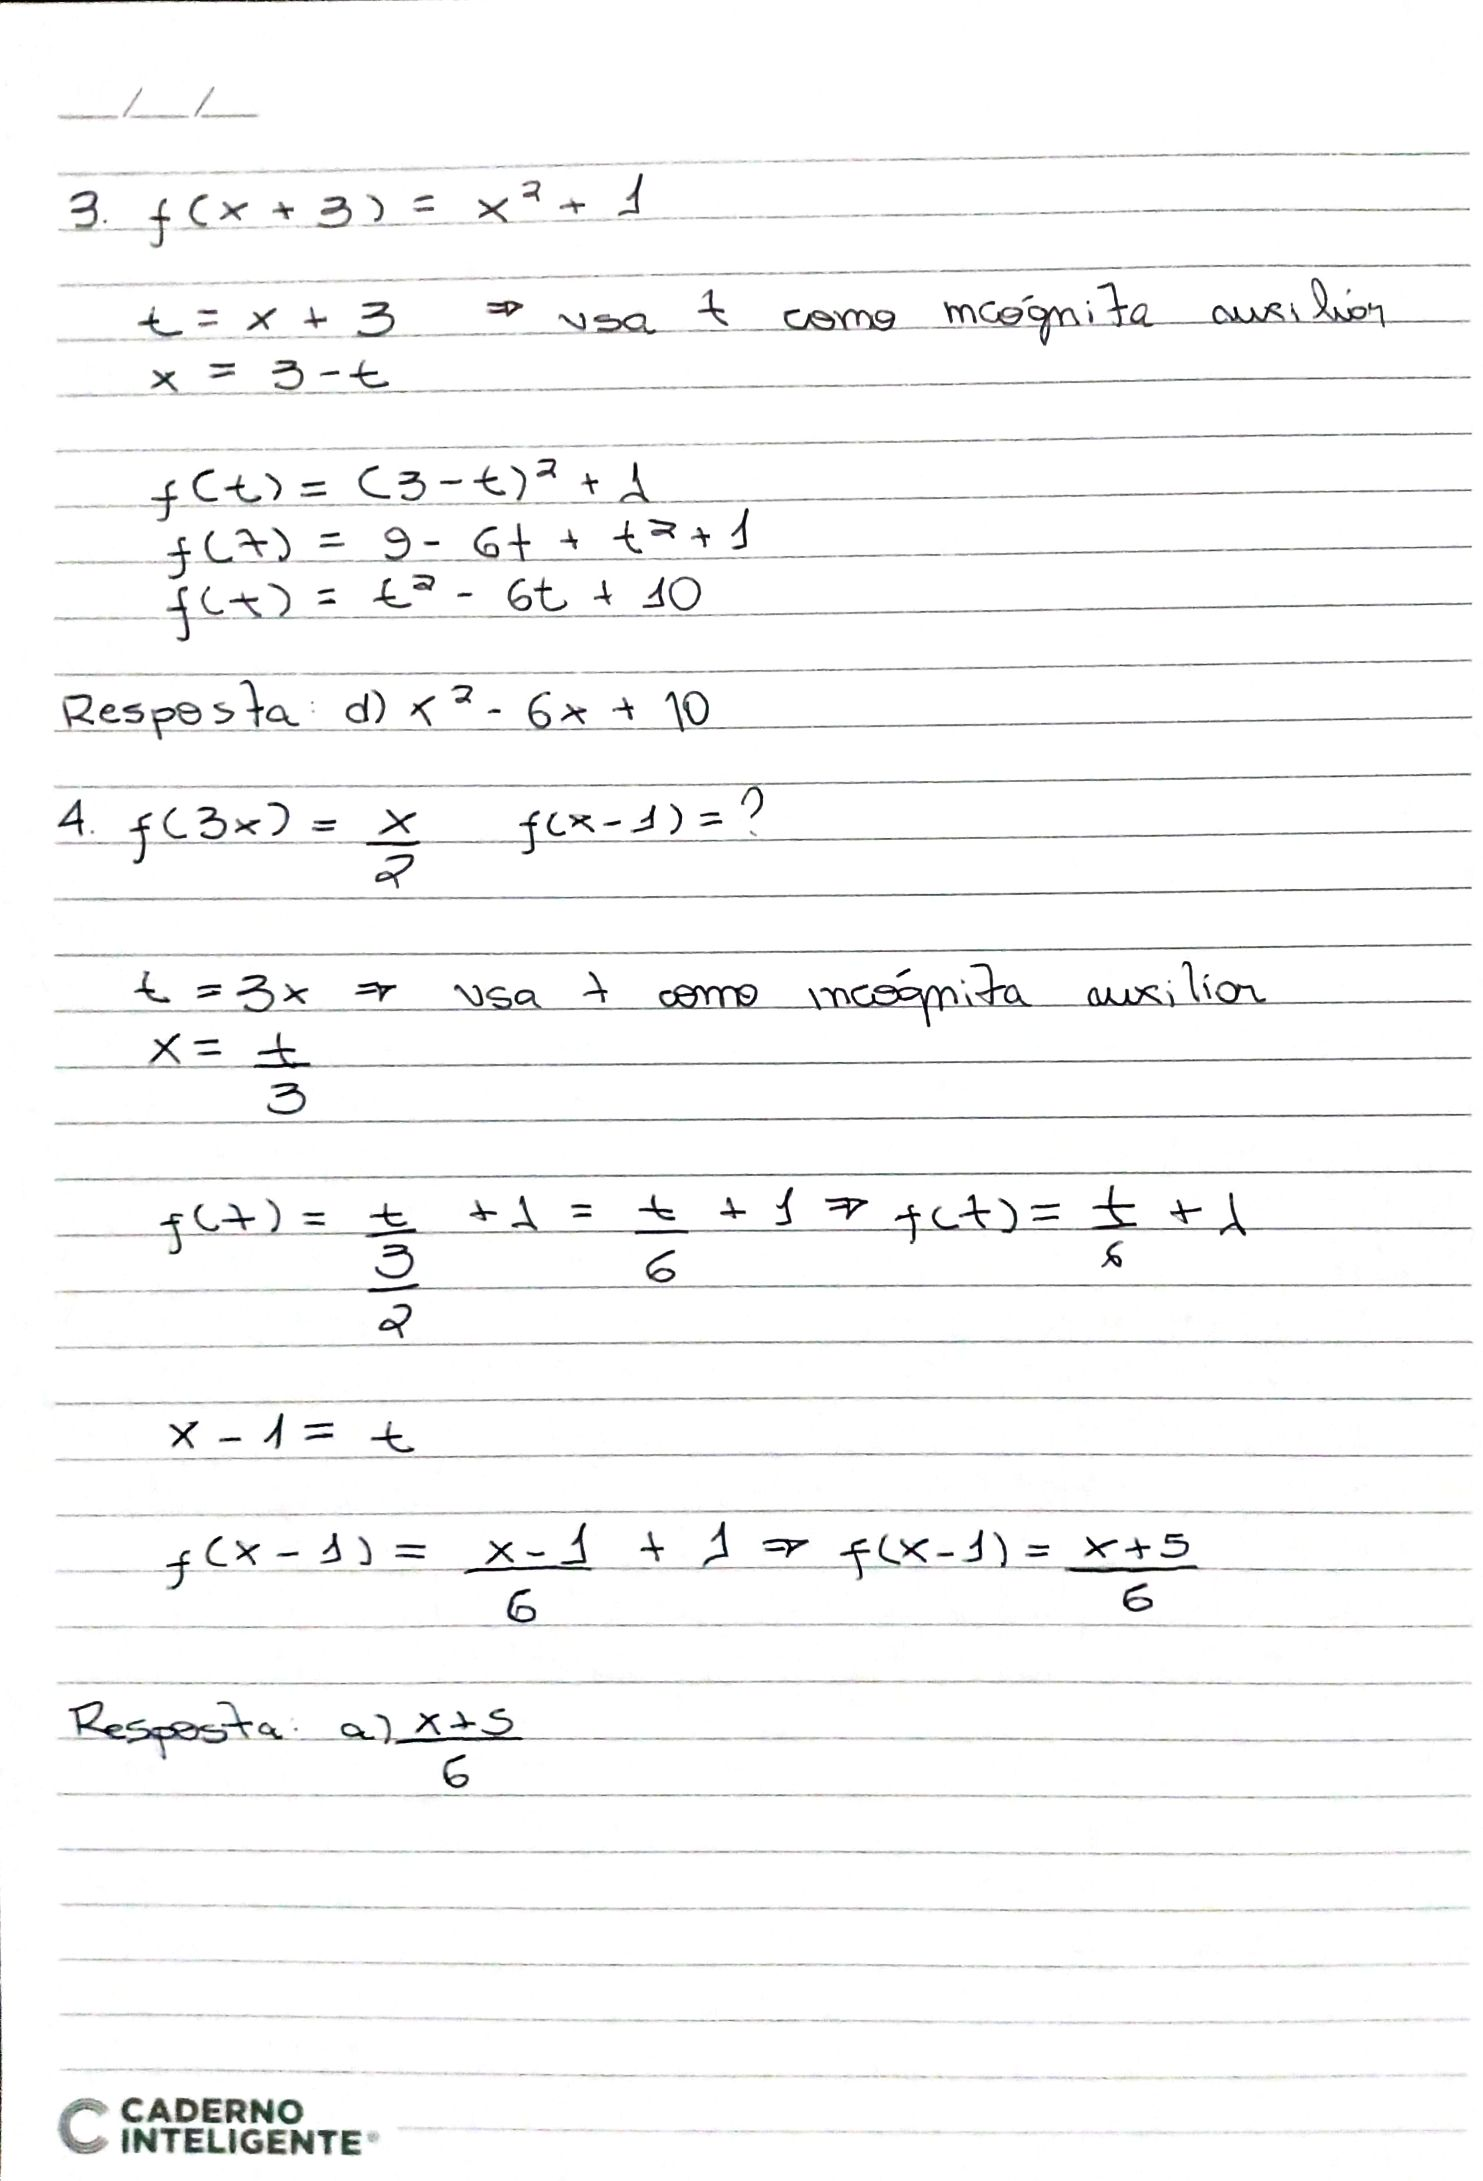
\includegraphics[scale=0.23]{pagina12.jpg}
\end{figure}

\begin{figure}[H]
  \centering
  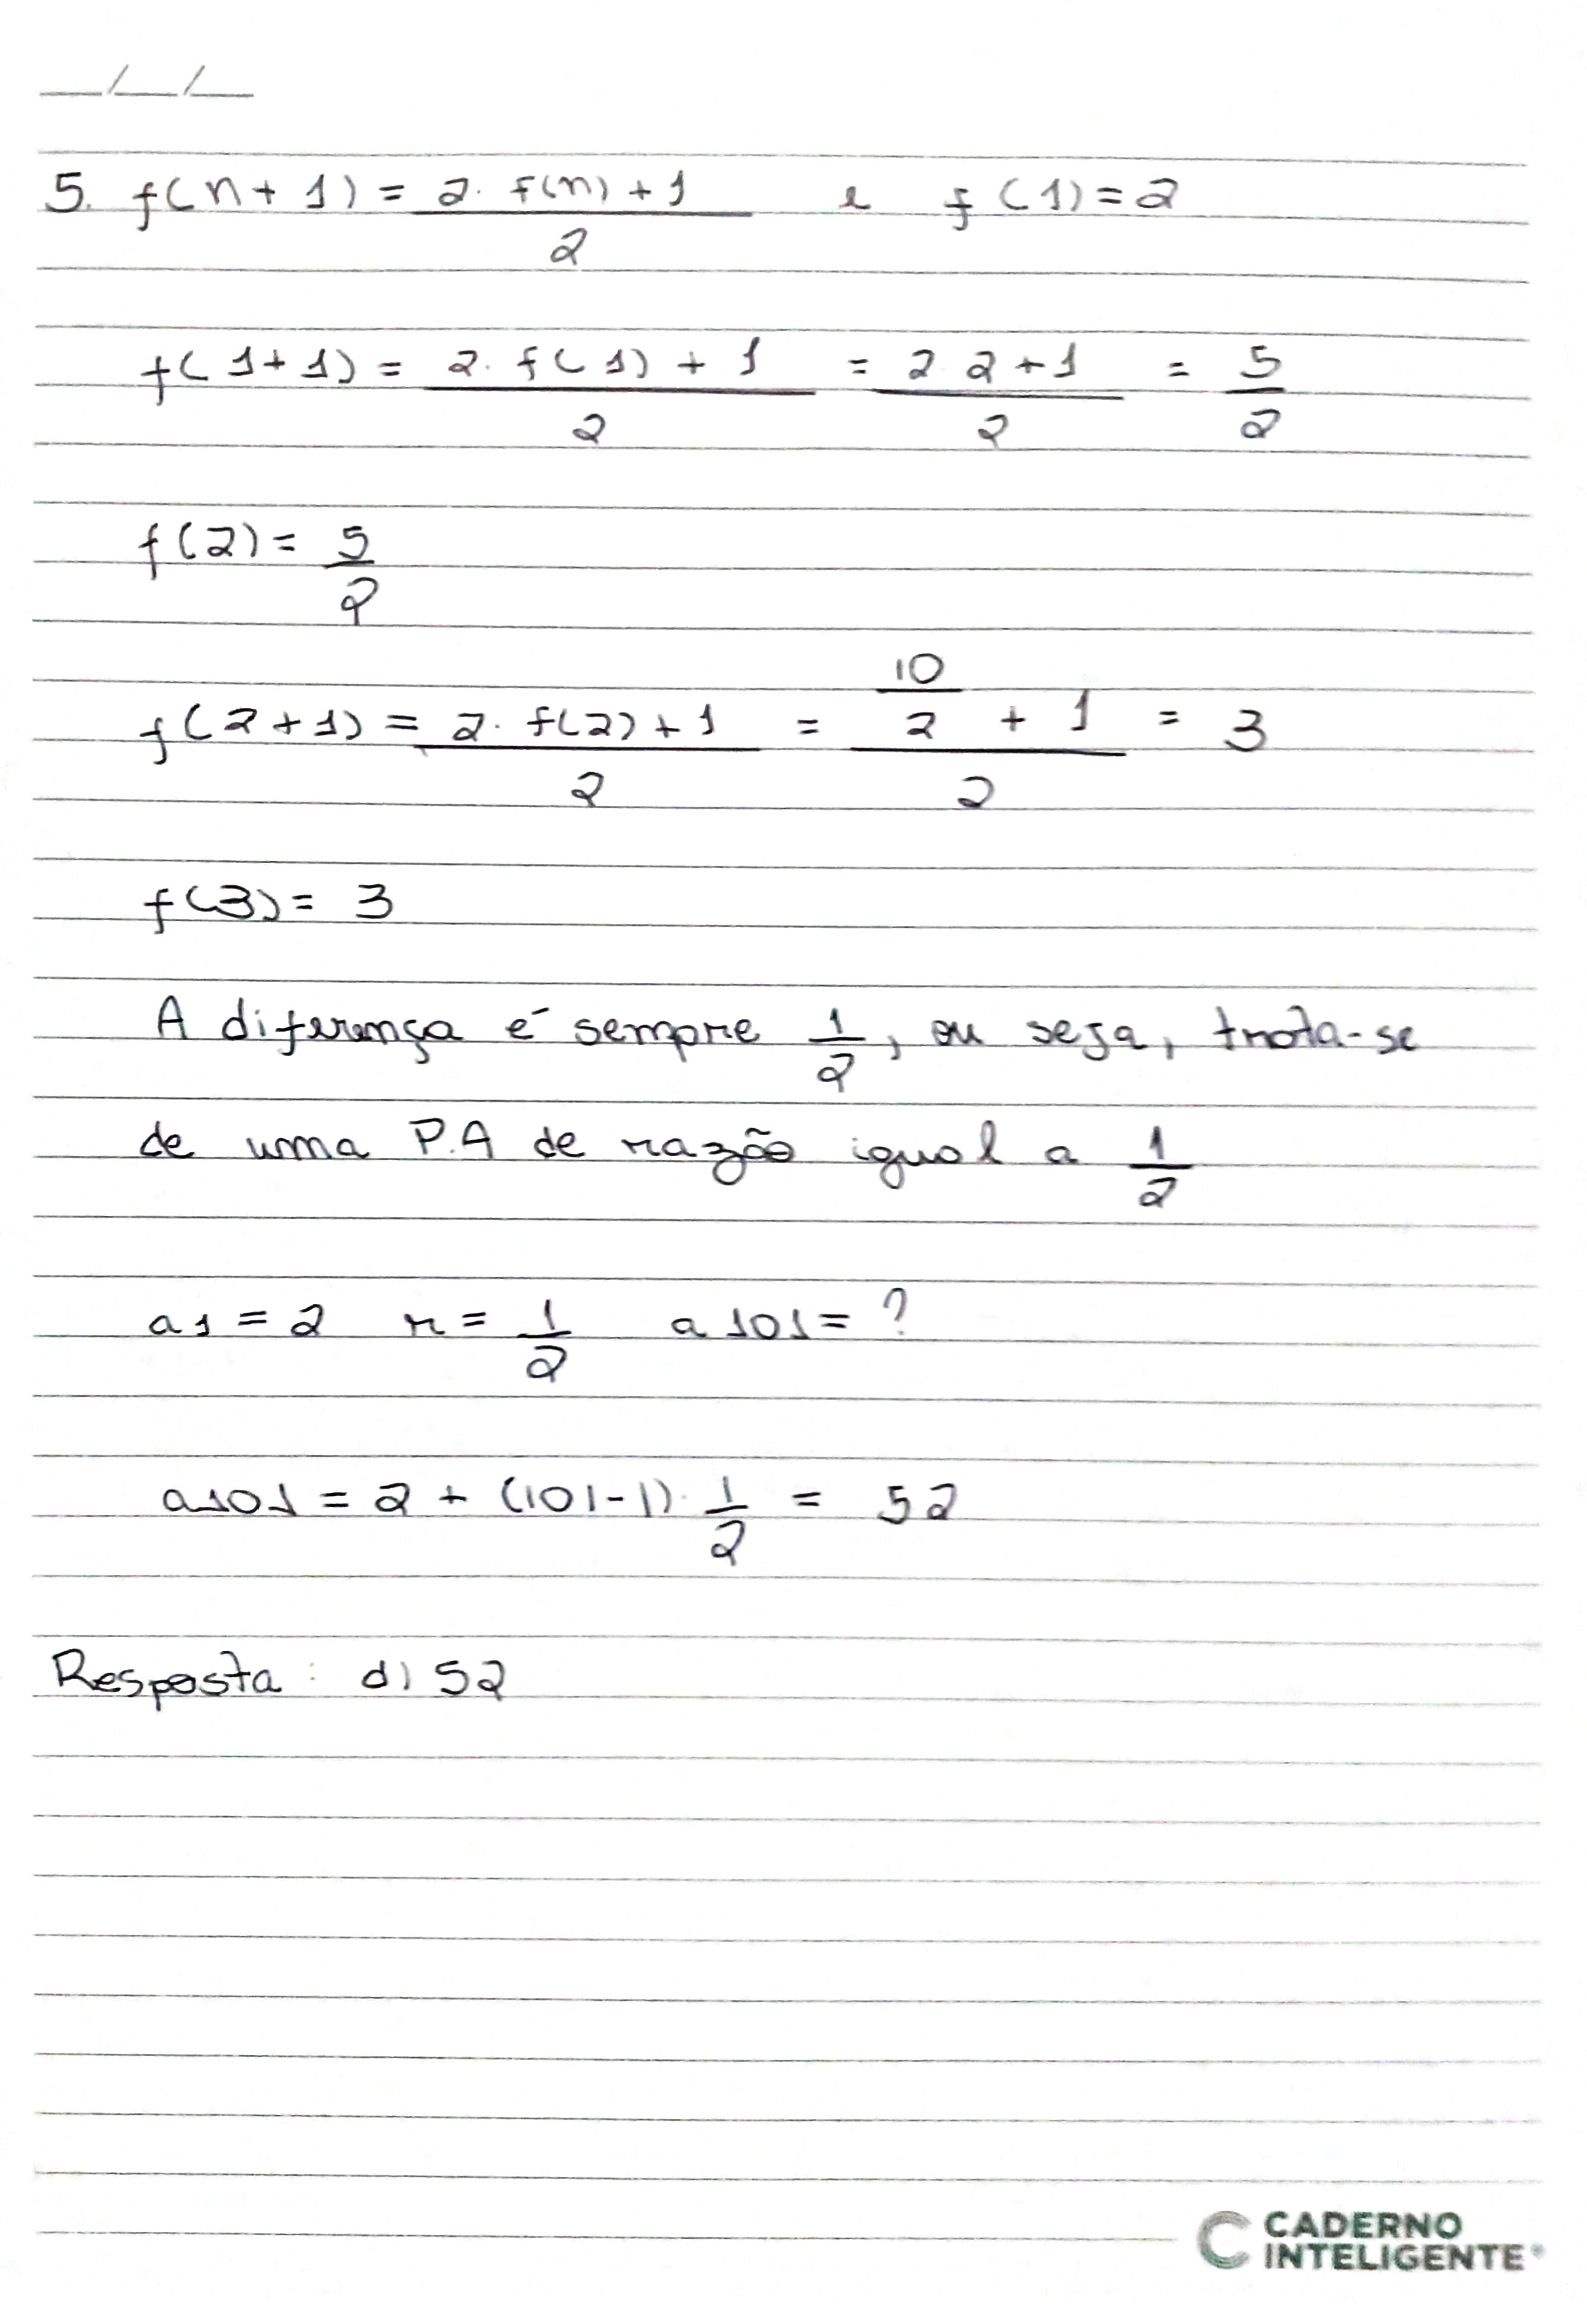
\includegraphics[scale=0.23]{pagina13.jpg}
\end{figure}

\begin{figure}[H]
  \centering
  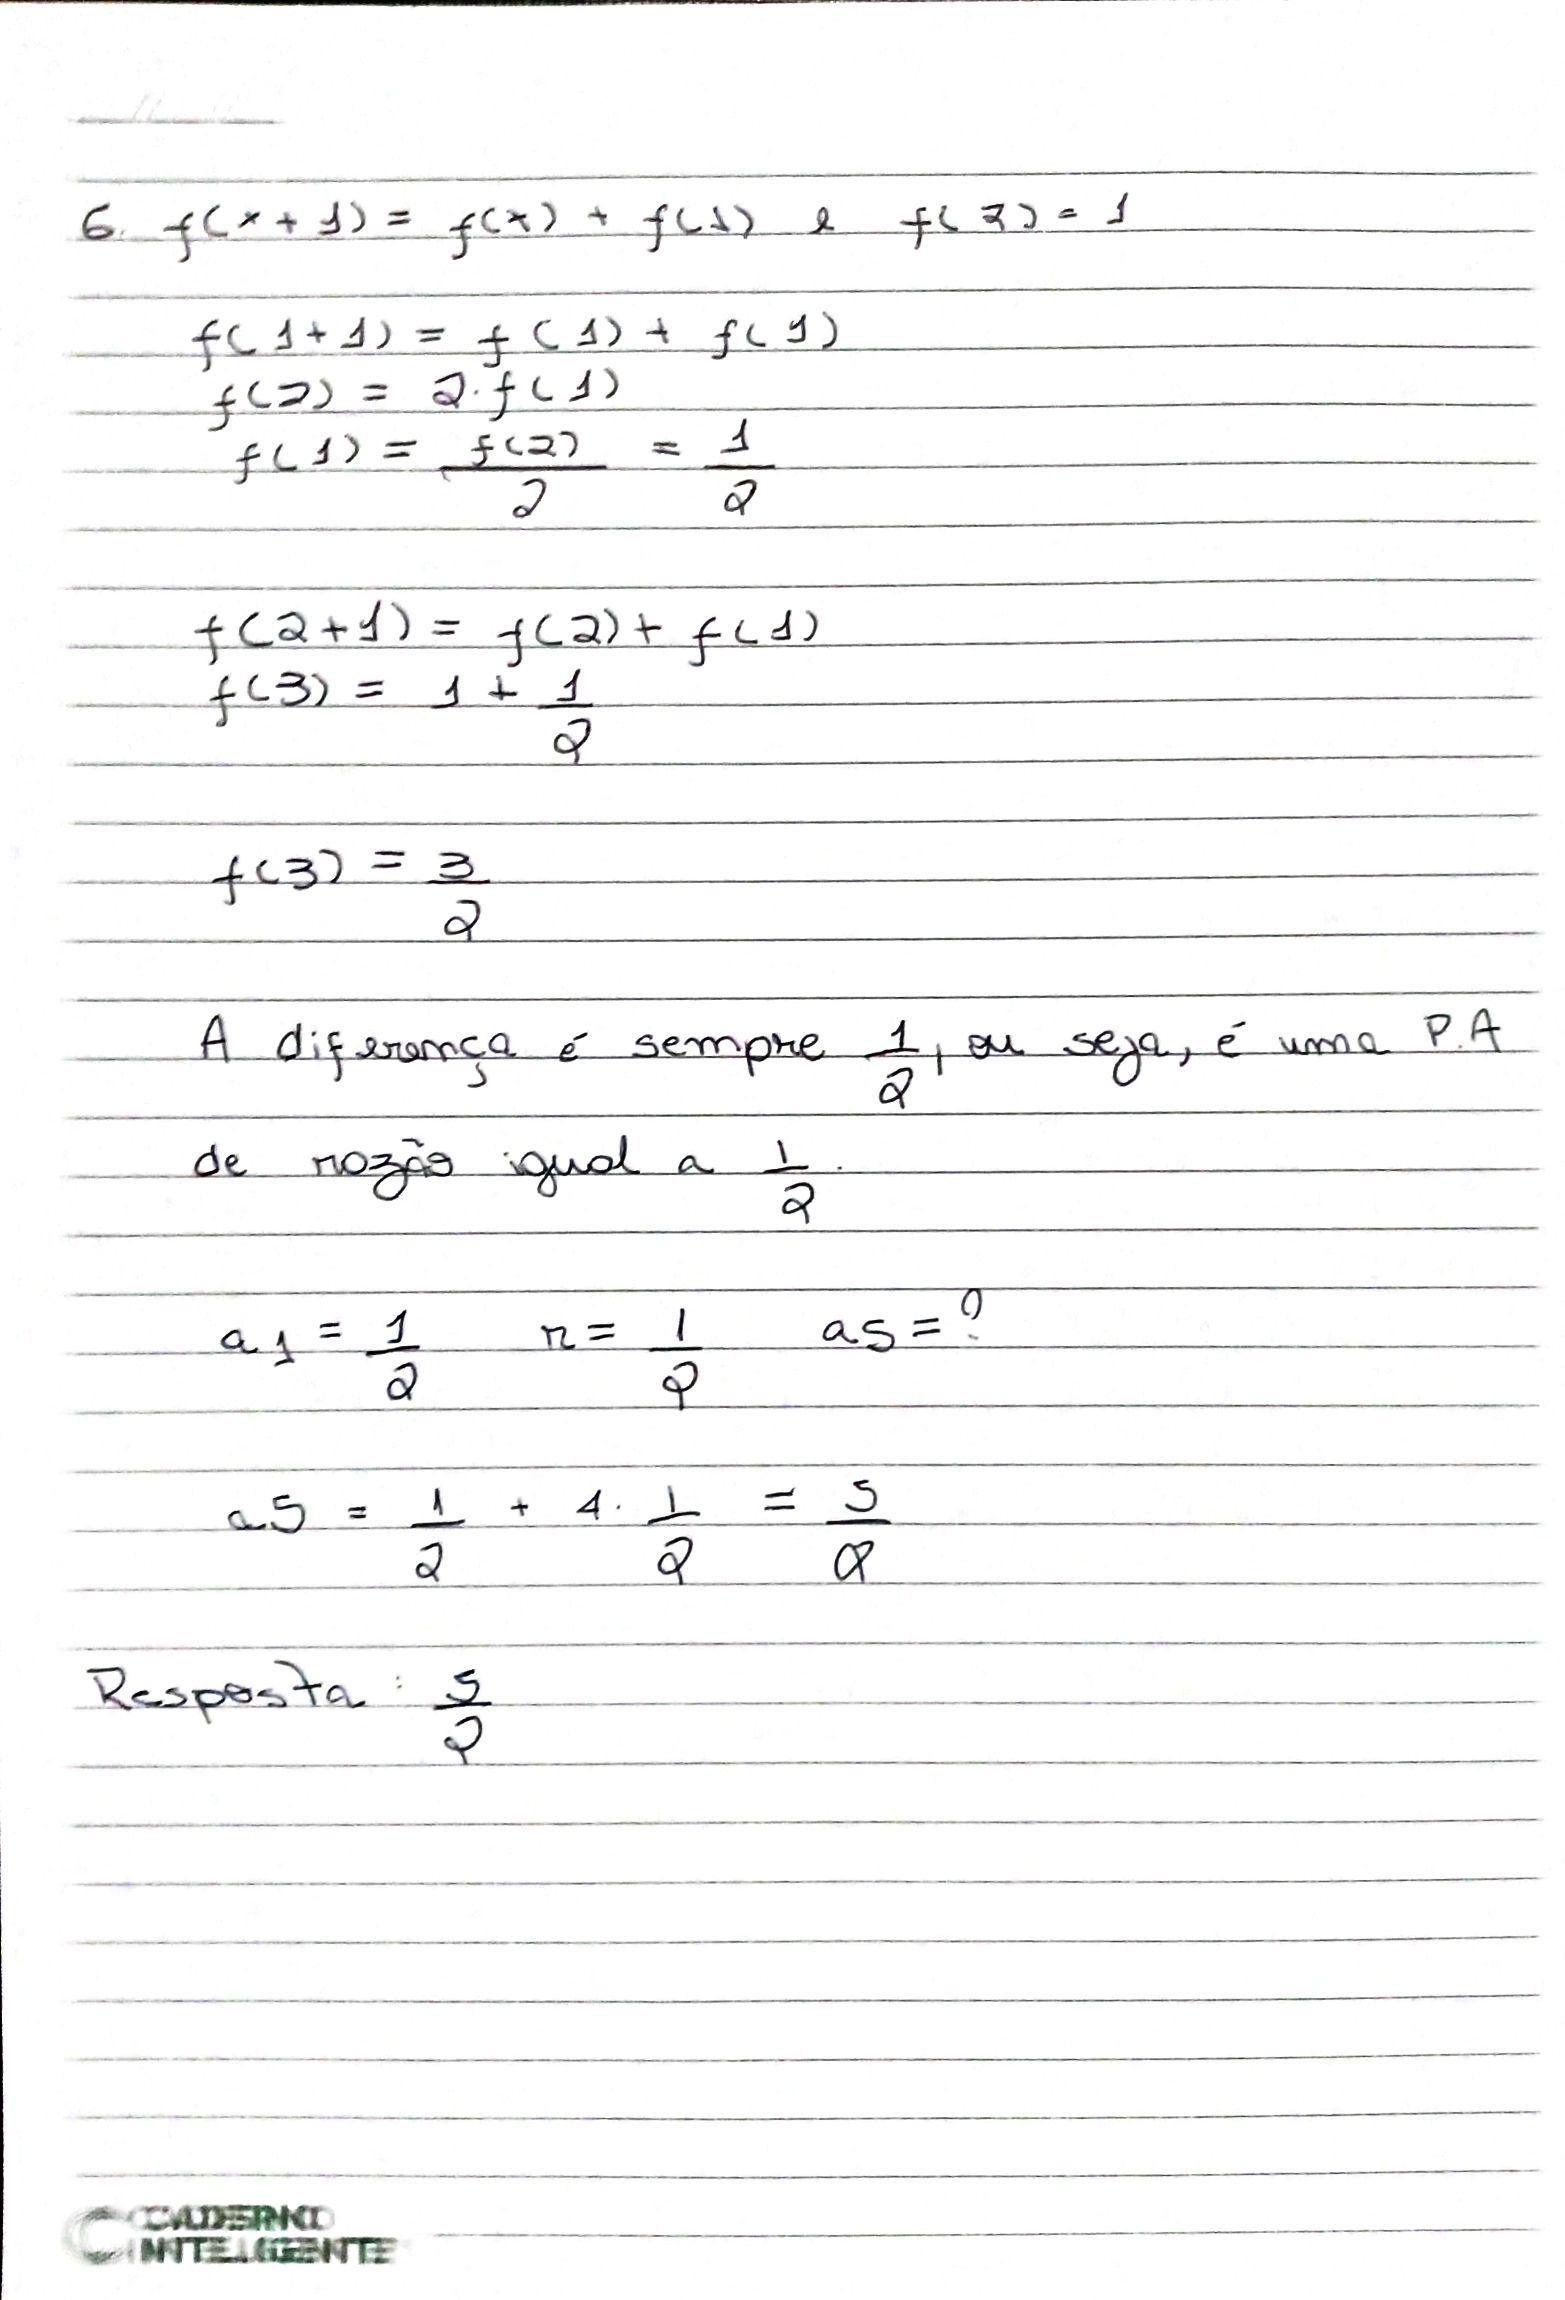
\includegraphics[scale=0.23]{pagina14.jpg}
\end{figure}

\begin{figure}[H]
  \centering
  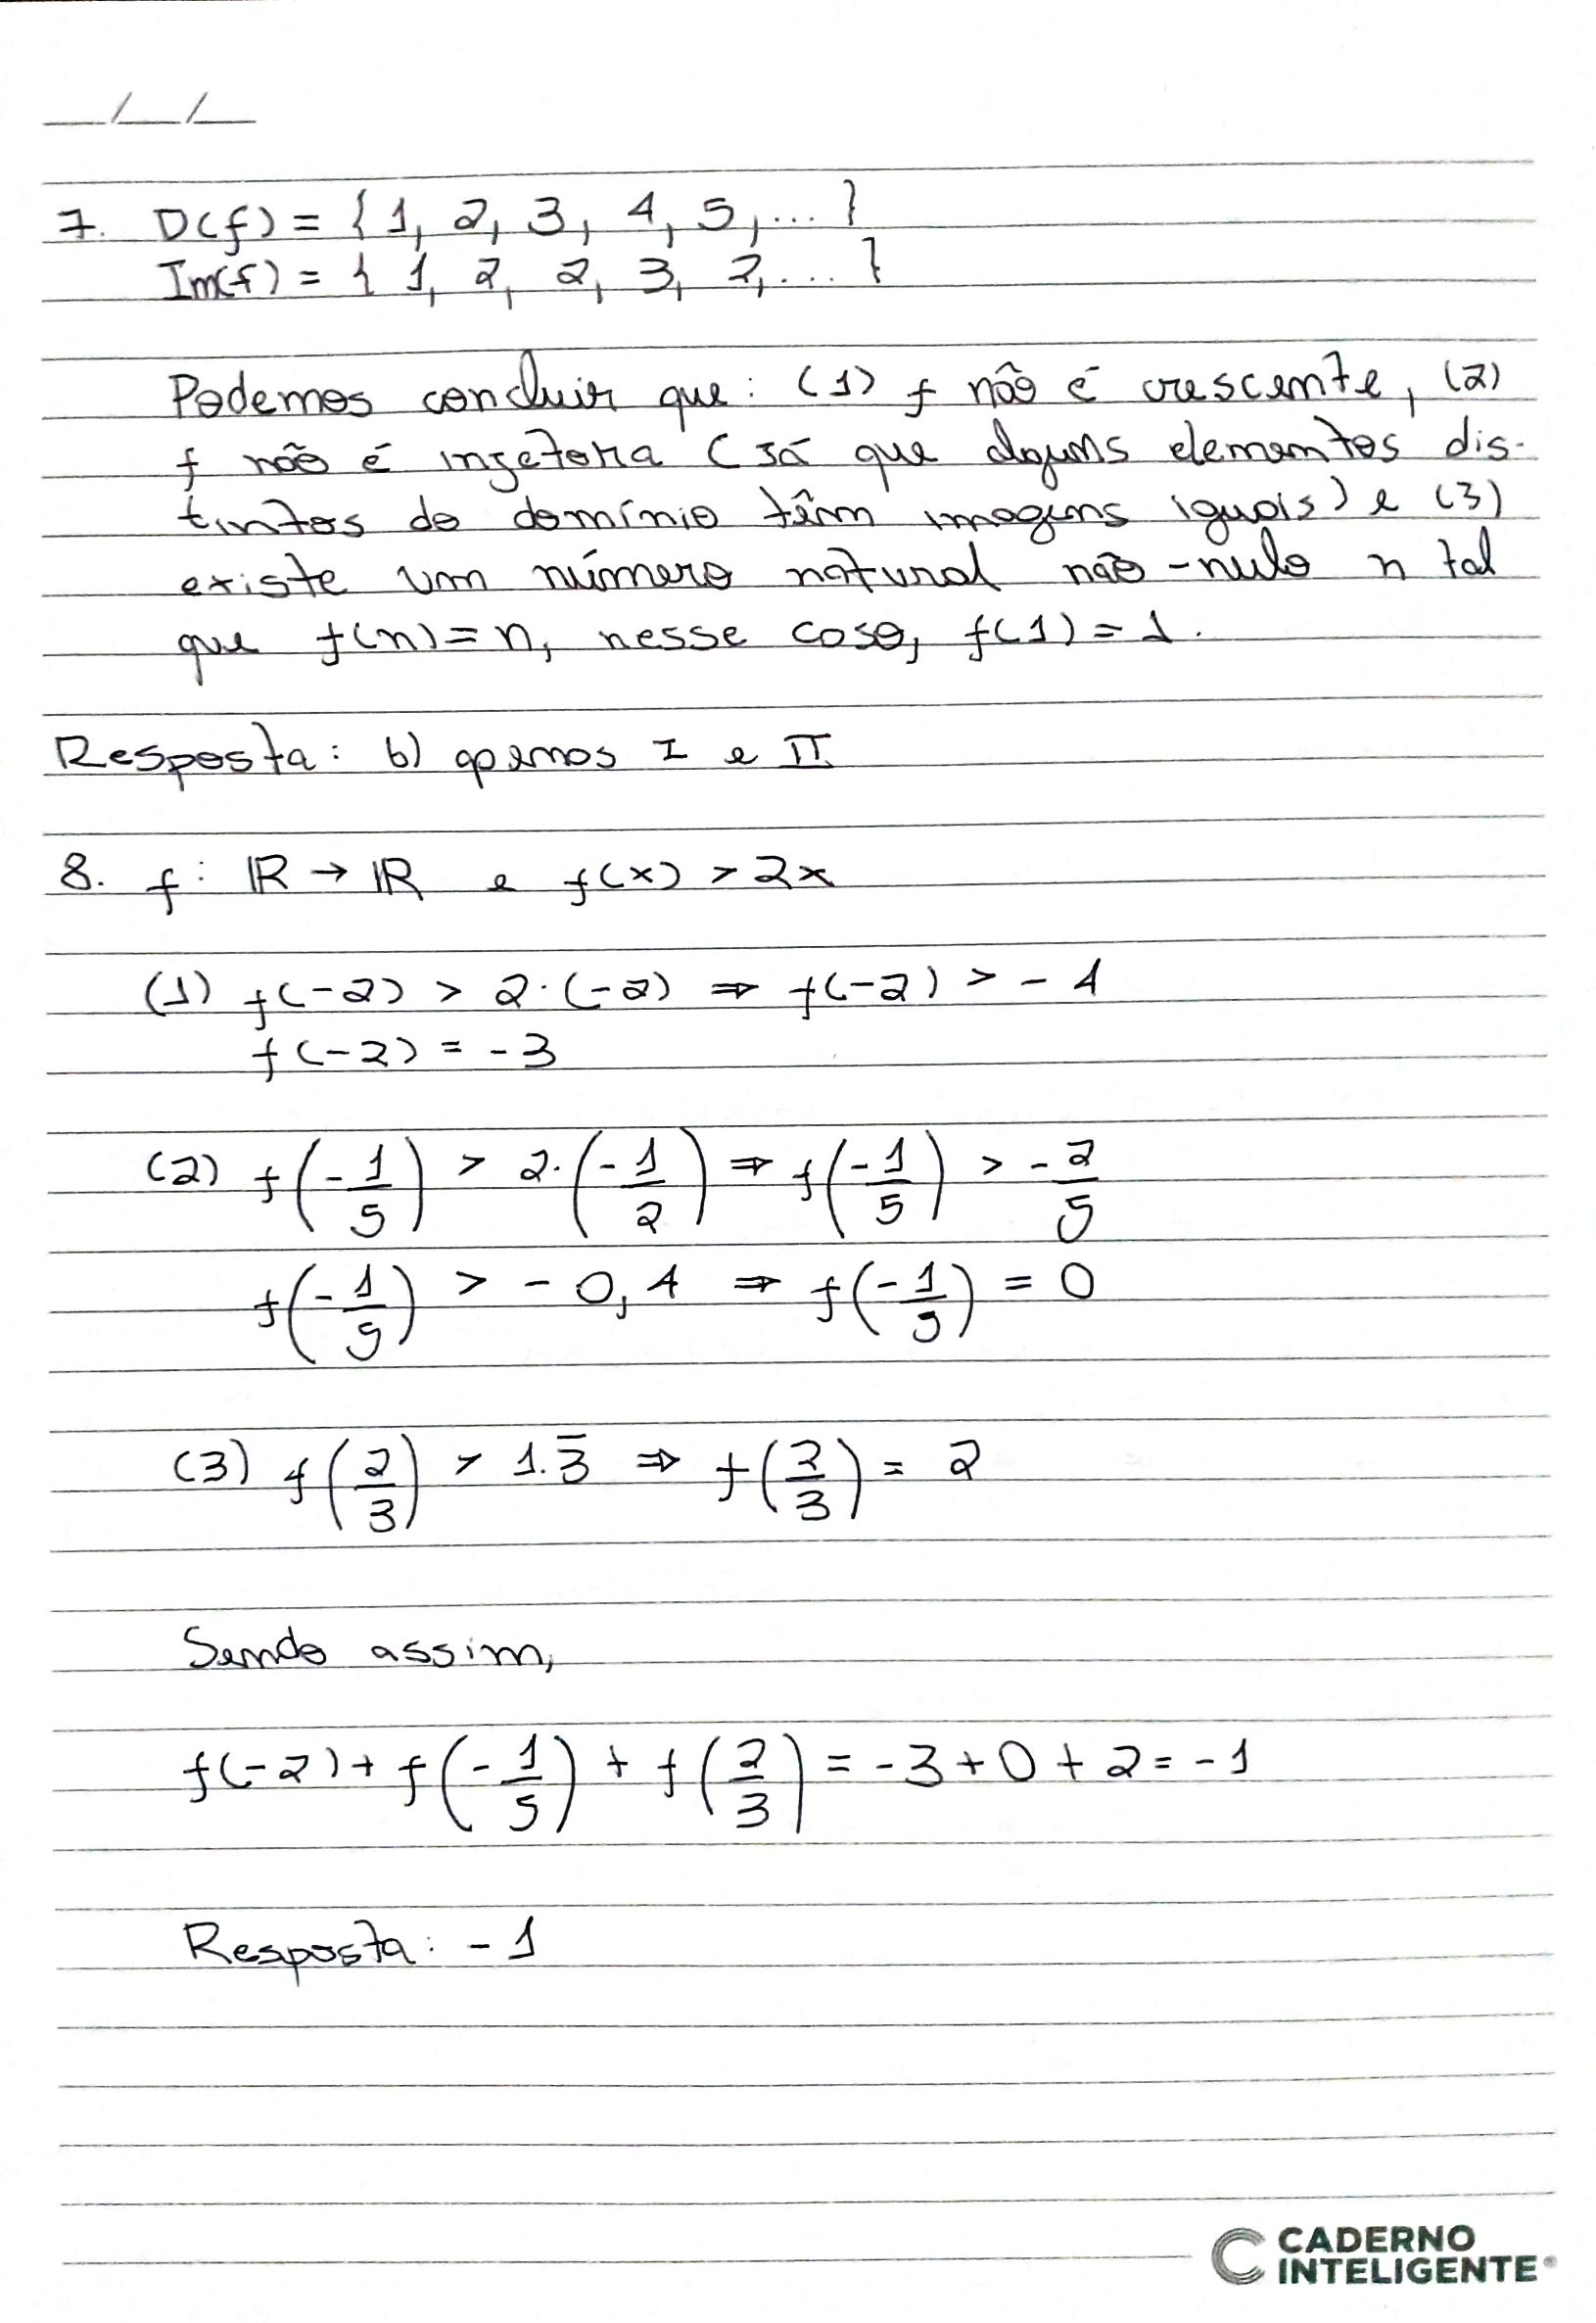
\includegraphics[scale=0.23]{pagina15.jpg}
\end{figure}

\begin{figure}[H]
  \centering
  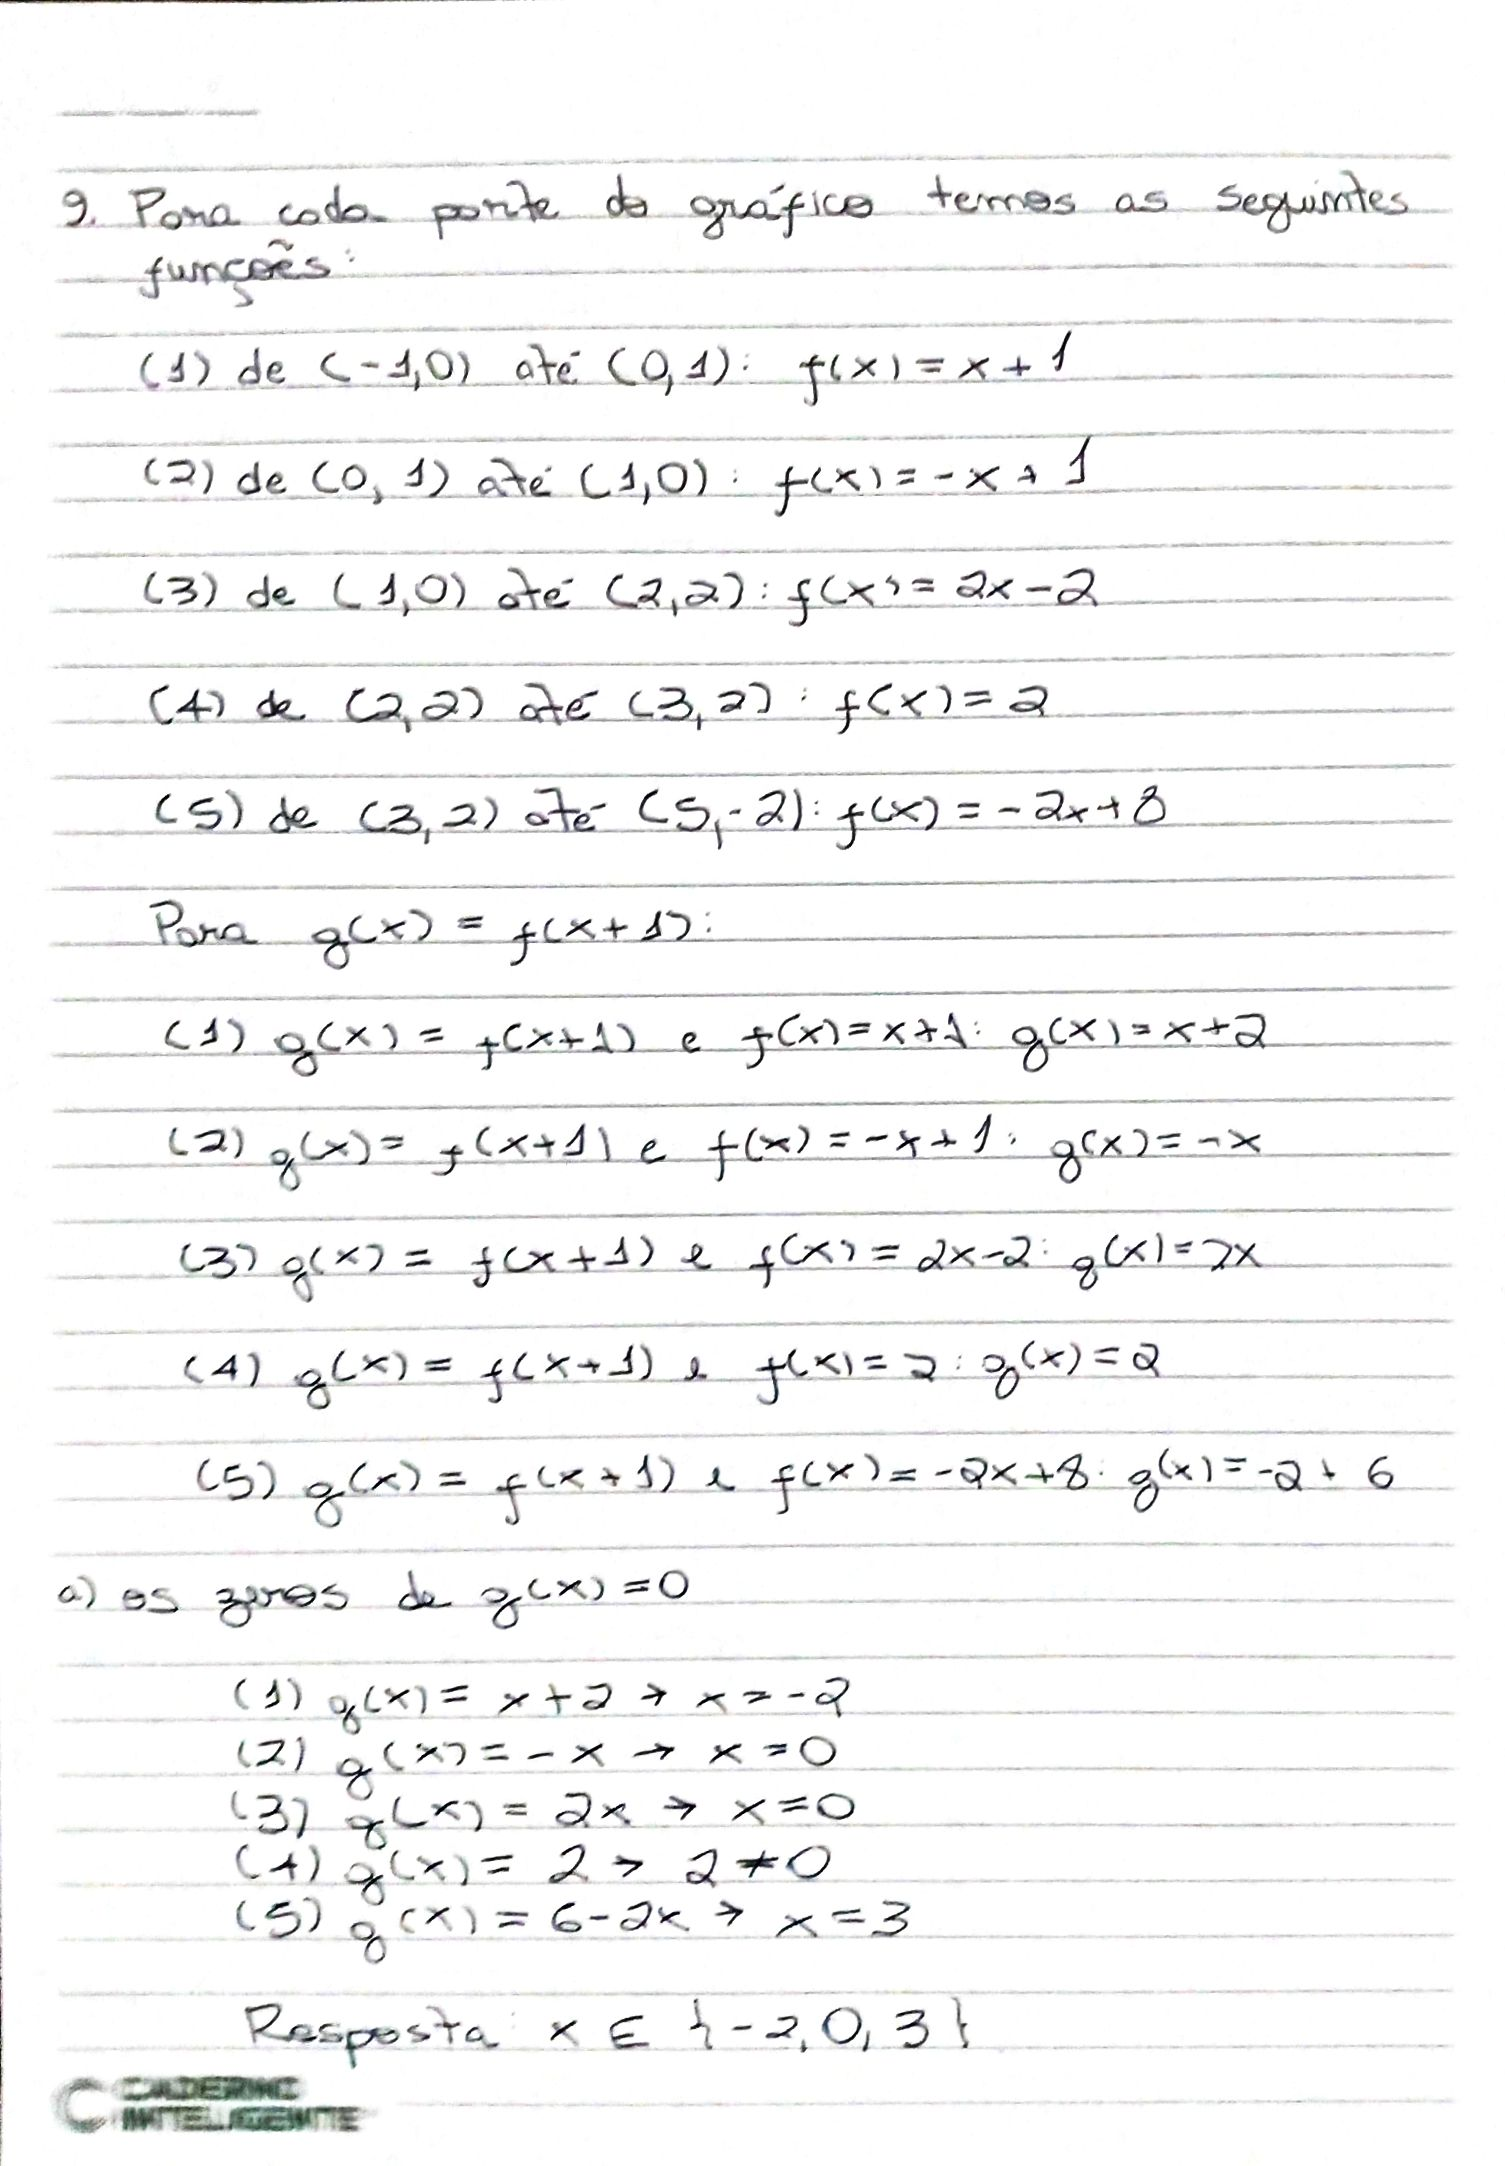
\includegraphics[scale=0.23]{pagina16.jpg}
\end{figure}

\begin{figure}[H]
  \centering
  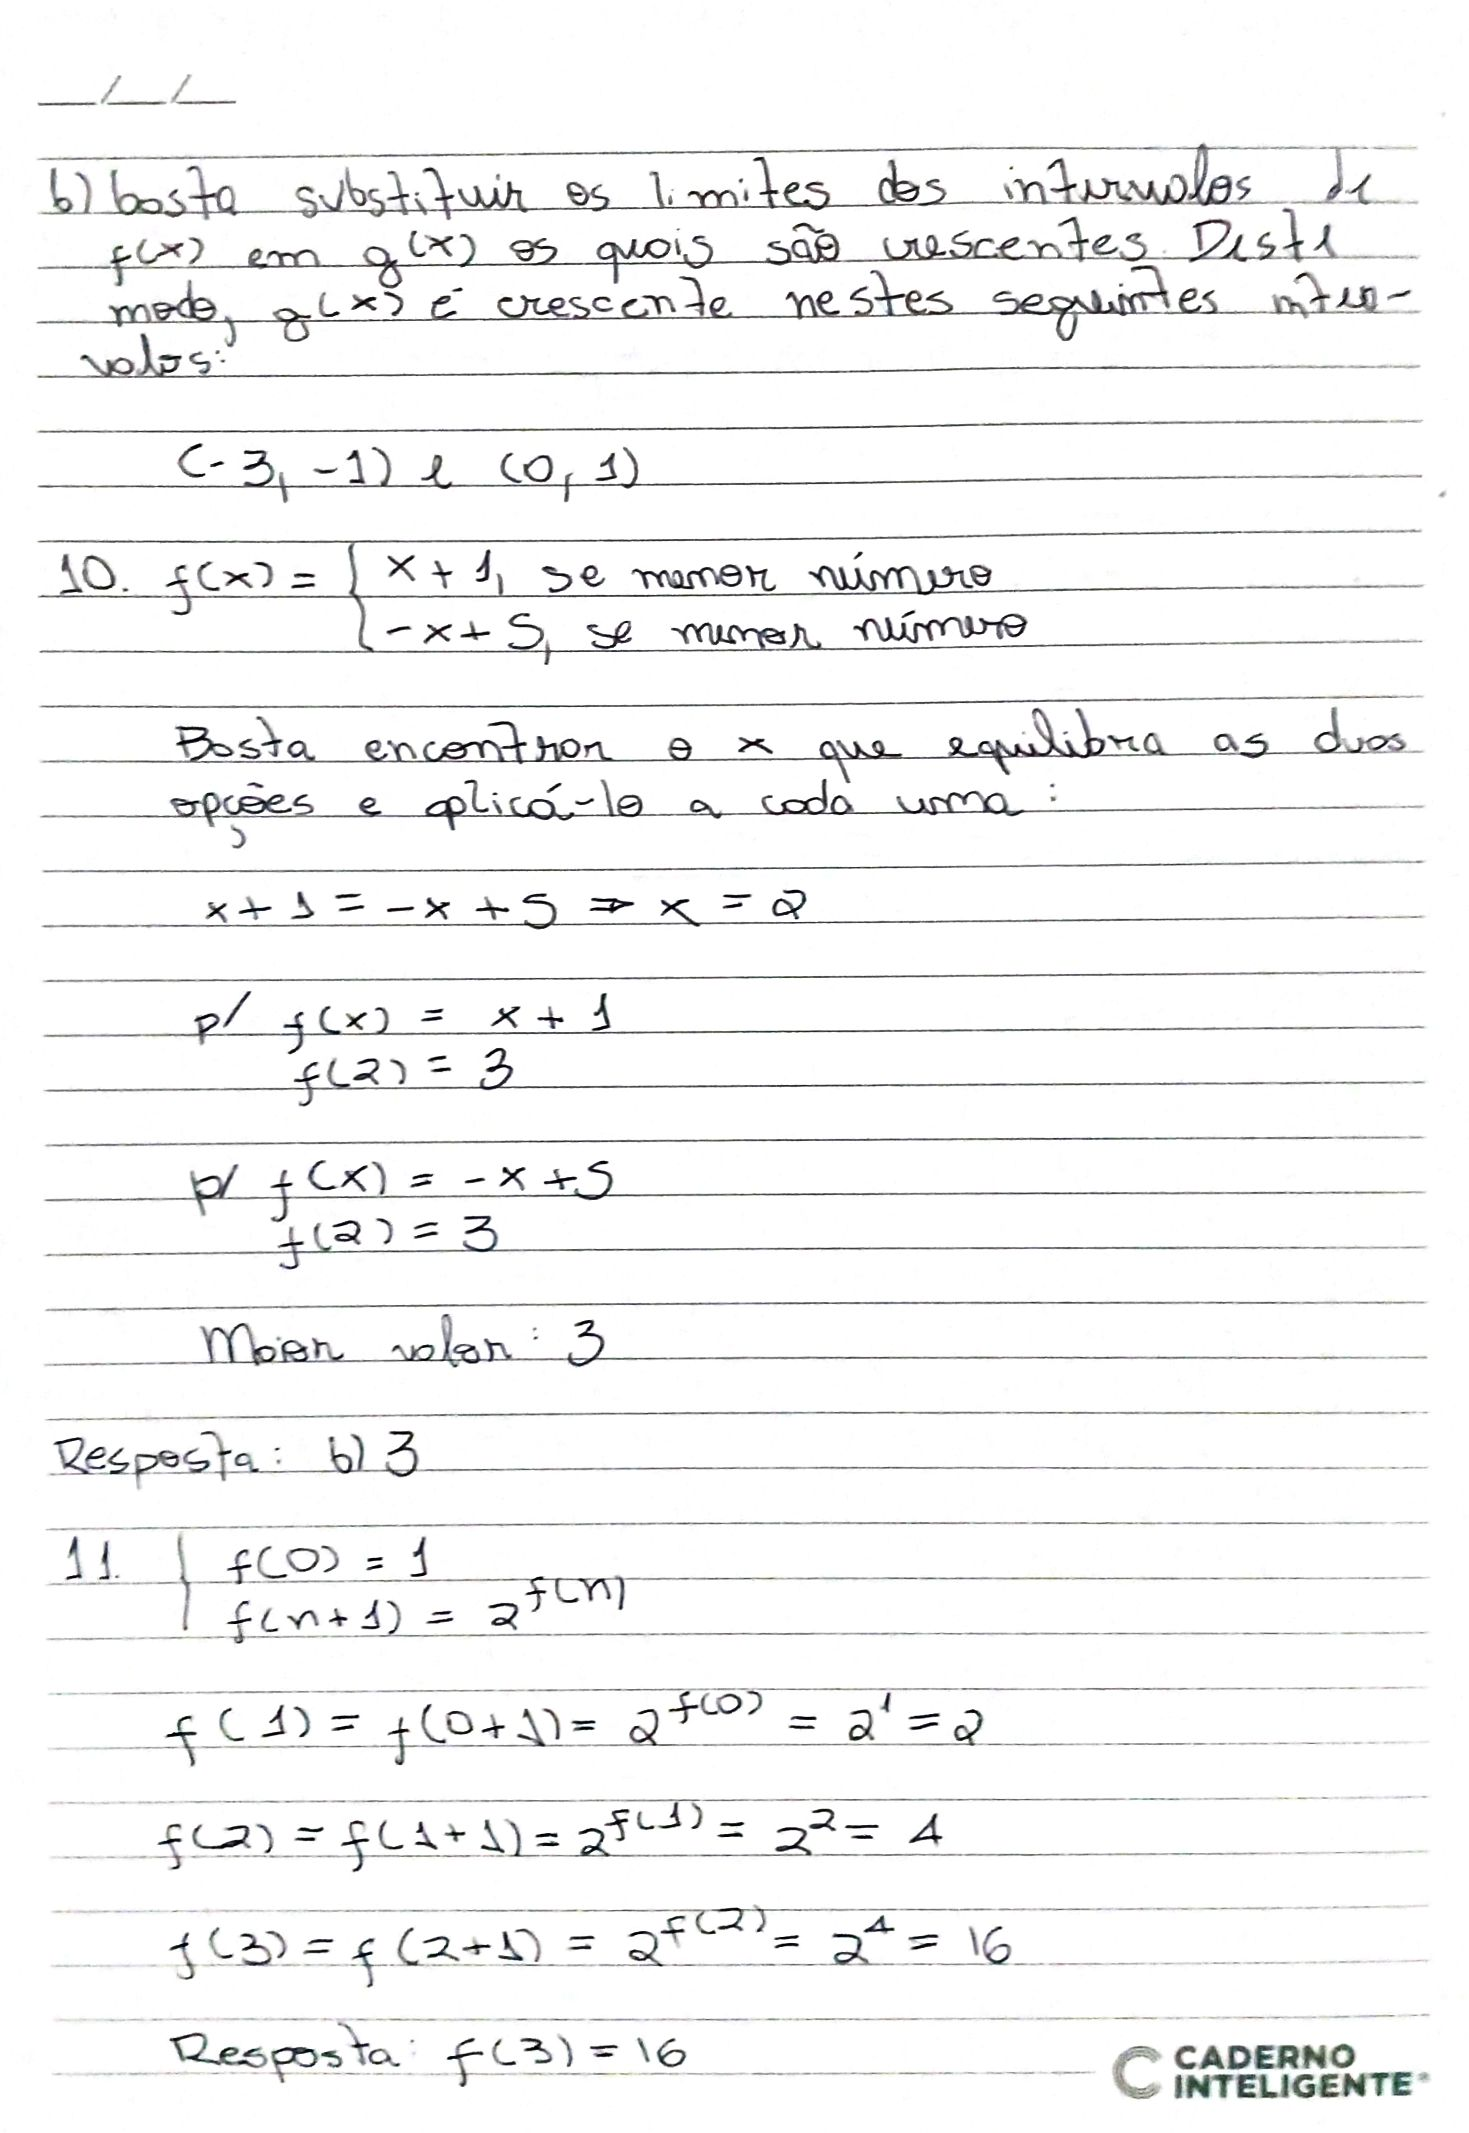
\includegraphics[scale=0.23]{pagina17.jpg}
\end{figure}

\begin{figure}[H]
  \centering
  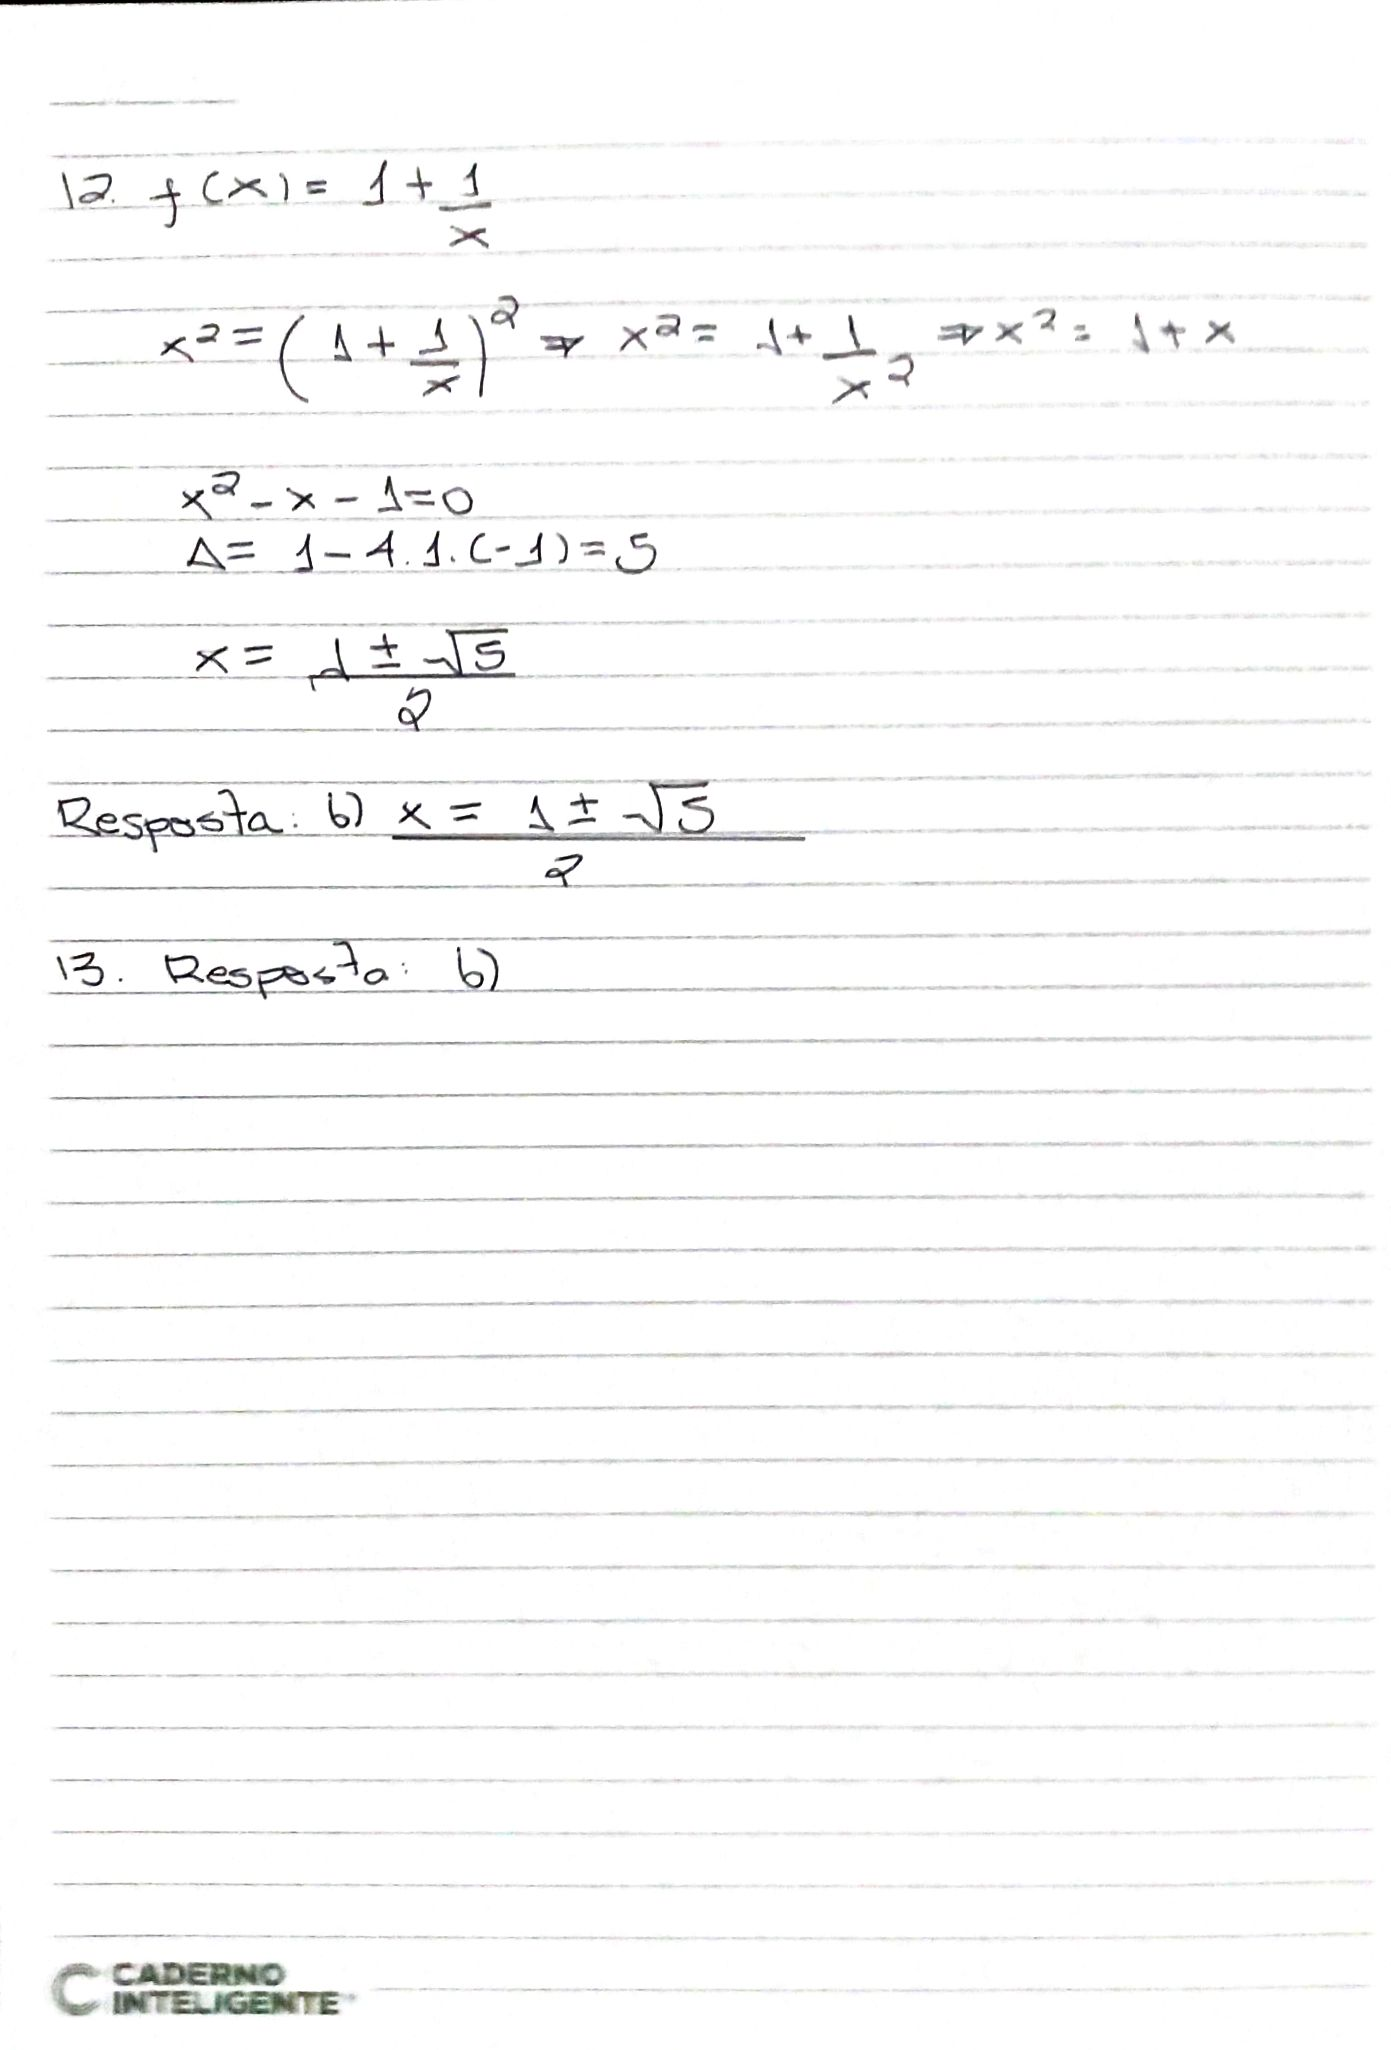
\includegraphics[scale=0.23]{pagina18.jpg}
\end{figure}

\end{document}
